\documentclass[12pt]{article}
\usepackage{tgtermes}
\usepackage[margin=1in]{geometry}
\usepackage{amsmath,amssymb,amsthm}
\usepackage{graphicx}
\IfFileExists{booktabs.sty}{\usepackage{booktabs}}{\newcommand{\toprule}{\hline}\newcommand{\midrule}{\hline}\newcommand{\bottomrule}{\hline}}
% hyperref unusable here (pdftexcmds.sty missing); url.sty is present and breaks long URLs
\usepackage{url}
% float.sty missing; [H] placements rewritten to [!htbp]
% setspace.sty missing; approximating onehalfspacing
\providecommand{\onehalfspacing}{\linespread{1.25}\selectfont}
\newtheorem{theorem}{Theorem}
\newtheorem{proposition}{Proposition}
\newtheorem{definition}{Definition}
\newtheorem{lemma}{Lemma}
\title{Computational Limits and Robustness of Predicting\\Developmental Cell-Fate Landscapes:\\Simulation, Published Networks and Measured Gradients}
\date{September 2026}
\onehalfspacing
\begin{document}
\maketitle
\begin{abstract}
\noindent When can computation predict developmental cell-fate landscapes, and at
what cost in information and robustness? We examine three mixed-evidence studies: synthetic pattern simulations, published regulatory models and public measured gradients, organized as one argument: (A) the tested dispersion-curve CNN does not improve held-out wavenumber prediction, and a physics check on measured
transport parameters shows \emph{where} self-organization can operate at all;
(B) fate robustness depends on transition dynamics, perturbation kernel and
starting measure, with ranking reversals in a published floral model; (C) supervised profile decoding is evaluated against specified empirical comparators, without measuring biological readout requirements. Study A simulates Turing reaction--diffusion
morphogen patterning (Gierer--Meinhardt kinetics) and measures a systematic,
statistically robust \emph{beyond-onset wavenumber upshift}: simulated patterns
select wavenumbers 15--60\% above the linear fastest-growing mode, with the
largest deviations at intermediate distance from onset; we show honestly that
the tested convolutional surrogate on dispersion features fails to improve on the linear prediction ($n=171$ simulations). This is not an impossibility result for other features, estimators or training designs. Study B analyses the published
Drosophila segment-polarity Boolean network (Cell Collective id-021) by exact
attractor enumeration under all eight external signalling conditions,
reproduces the published bistability, quantifies the wild-type basin as
$0.77\%$ of the synchronous state space, and measures the sample complexity of
learning the basin boundary (graph neural network vs.\ multilayer perceptron).
Study C analyses 676 real Bicoid-GFP morphogen gradients and 2{,}180
gap-gene immunofluorescence embryo records (Liu, Morrison \& Gregor, PNAS
2013): we (i) reproduce the gradient length scale under the authors' own
fitting window, (ii) quantify a dosage-coupled length-scale effect that is
concentrated in the anterior embryo (Spearman $\rho=0.36$, $p=8\times10^{-16}$
in anterior windows; absent in the authors' posterior window), (iii) beat the
published threshold model of cephalic-furrow positioning with a one-dimensional
convolutional decoder (RMSE 2.38\% egg length vs.\ 4.94\% egg length,
held-out fly lines; paired bootstrap CI for the gain $[1.99,3.11]\%$ EL), and
(iv) show that positional decodability from Hb+Eve expression improves with
maternal \emph{bcd} dosage (6.21\% vs.\ 9.91\% EL median error; bootstrap CI
$[3.00,4.40]\%$ EL). Two headline measurements tie the studies together: a \emph{developmental fragility index}
for the segment-polarity network ($F=0.500$; exactly half of all 1{,}792 single-node perturbations of
wild-type-basin states destroy the wild-type outcome, concentrated entirely in the CI/EN axis, with
seven clamp interventions that abolish the basin and six that double it) and a \emph{minimum-information
threshold} for morphogen readout (cephalic-furrow position is decodable below the published benchmark
from a single measured point of the Bicoid gradient, 4.29\% vs 4.94\% EL for the true-dose comparator). The measured-amplitude comparator in the same benchmark has lower RMSE, 2.8566\% EL, so the one-point result does not beat all threshold alternatives. Negative results (a retracted small-sample surrogate win,
single-exponential sufficiency, degenerate basin classification) are reported
alongside positive ones, each with its positive interpretation. All code, tests, data manifests and result files are
public at the project repository.
\end{abstract}
\tableofcontents
\newpage
\section{Introduction}
\subsection{Digital embryos}

A \emph{digital embryo} is a computational reconstruction of a developmental
process that is close enough to the underlying biology to be wrong in
interesting ways. The promise of the field is that cheap computation can
replace some expensive experimentation: simulate the morphogen, the network,
or the tissue, and reserve the bench for questions the simulation cannot
answer. The peril is equally well known --- a simulation unconstrained by real
measurements will happily reproduce whatever its author expected. This report
takes the second half of that sentence seriously. Three classical model
systems of developmental patterning are rebuilt computationally, and every
quantitative claim is tied to real, accession-level public data: published
per-embryo morphogen measurements, a published gene-regulatory network model,
and published quantitative benchmarks. Where our computation contradicts an
initial expectation --- including our own earlier, stronger claims --- we say
so in the body of the report, not in a footnote.

The three studies correspond to the three great patterning problems of the
fly embryo, at three scales:

\begin{enumerate}
\item \textbf{Turing pattern selection (Study A).} Reaction--diffusion
systems of the type proposed by Turing \cite{turing1952} and instantiated by
Gierer and Meinhardt \cite{gierer1972} amplify a band of spatial wavelengths
out of noise. Linear theory predicts which wavenumber grows fastest; what the
\emph{saturated, nonlinear} pattern actually selects is a subtler question.
We measure the selected wavenumber across a parameter sweep and ask whether
the deviation from linear theory is itself predictable.
\item \textbf{Gene-network attractors (Study B).} The segment-polarity
network of \emph{Drosophila} is one of the best-studied Boolean models in
systems biology \cite{vondassow2000,albert2003}. We take the published
14-node Boolean model (Cell Collective id-021 \cite{helikar2012}) as ground
truth, enumerate its attractors exactly under all eight external signalling
conditions, measure the size of the wild-type basin of attraction, and ask
how much data a learning algorithm needs to recover the basin boundary.
\item \textbf{Morphogen positional information (Study C).} The Bicoid
morphogen gradient of the early fly embryo is the canonical example of
positional information \cite{wolpert1969,gregor2007}. Using the 676
per-embryo gradients and 2{,}180 immunofluorescence embryo records published
by Liu, Morrison and Gregor \cite{liu2013}, we (i) reproduce their gradient
length-scale measurements, (ii) test how the length scale depends on maternal
gene dosage, (iii) attack their threshold model of cephalic-furrow
positioning with a learned decoder, and (iv) measure how much positional
information gap-gene expression patterns carry under different dosages.
\end{enumerate}

\subsection{Why these three}

The three problems are independent in method but connected in spirit: each
asks where spatial order comes from, and each has a quantitative published
reference point that a computation can fail to meet. Study~A's reference is
the linear dispersion relation itself --- a prediction made by mathematics,
not by a measurement, which makes it the cleanest possible benchmark to break.
Study~B's reference is a published, curated, executable model: if our
attractor enumeration disagreed with it, the disagreement would be
diagnosable down to a single update rule. Study~C's references are the
hardest kind: numbers measured on real embryos, with real noise, by another
laboratory \cite{liu2013,petkova2019,gregor2007}.

\subsection{Summary of results}

Every number quoted here is computed by committed, tested code from committed
data, and re-computed when this report is built; the repository records the
exact pipeline. Section references point to full derivations and tables.

\begin{itemize}
\item \textbf{Study A (Sections \ref{sec:studyA}).} Across a 14-point sweep
of the activator decay rate, the saturated Gierer--Meinhardt pattern
systematically selects a wavenumber \emph{above} the linear fastest-growing
mode, by $14.7\%$ to $58.9\%$ (median $31\%$), with the largest relative
deviations at intermediate distance from onset --- not at threshold, where
amplitude-equation reasoning would have placed them. The deviation is real
(measured at steady state, verified against two lattice sizes) but it is
\emph{not} predictable from the linear dispersion curve by a convolutional
surrogate: a promising $n = 58$ pilot result ($+17.7\%$ held-out improvement)
\emph{failed to replicate} at $n = 171$ (CNN relative RMSE $0.292$--$0.295$
vs.\ $0.272$ for the linear formula alone). We retract the small-sample claim
and keep the phenomenon.
\item \textbf{Study B (Section \ref{sec:studyB}).} Exact attractor
enumeration of the published segment-polarity network under all eight
combinations of the external signals \textsc{hh}, \textsc{WG}, \textsc{SLP}
reproduces the published condition-dependent bistability exactly
\cite{albert2003}. The wild-type (\textsc{wg}-ON) basin occupies $0.77\%$ of
the synchronous state space under the wild-type signalling condition. The
basin boundary is learnable to $> 98\%$ test accuracy from only $\sim 60$
labelled states (of $2^{14}$), and a graph neural network matches or beats a
multilayer perceptron at every sample size; under naive uniform sampling the
classification task is degenerate (majority class accuracy $99.3\%$), which
we report as a cautionary result.
\item \textbf{Study C (Sections \ref{sec:studyC}--\ref{sec:gapdecode}).}
From 676 real Bcd-GFP gradients: the population length scale reproduces the
published value under the authors' fitting window ($\lambda_{\mathrm{median}}
= 0.189$ vs.\ published $0.165 \pm 0.007$ egg lengths \cite{liu2013}, with
our value on their exact window; the residual difference is discussed
honestly). The length scale \emph{increases with maternal bcd dosage}
(dosage-coupled length scale, DCLS): Spearman $\rho = 0.356$
($p = 7.9 \times 10^{-16}$) on anterior-weighted fitting windows, robust to
parametric refitting (OLS slope $+0.0117$ per dose, $95\%$ CI
$[0.0060, 0.0174]$, $p = 5.9 \times 10^{-5}$), and \emph{absent} on the
posterior-heavy window used in the original publication ($\rho = 0.071$,
$p = 0.12$) --- a window-sensitivity finding, not a contradiction. A
one-dimensional convolutional decoder predicts cephalic-furrow position from
the raw Bcd profile at $2.38\%$ egg length RMSE (held-out fly lines,
$R^2 = 0.854$), beating the published threshold model at $4.94\%$ EL by a
paired-bootstrap margin of $2.57\%$ EL, CI$_{95}$ $[1.99, 3.11]$
($p < 10^{-4}$). Finally, positional decodability from joint Hb+Eve
expression improves with dosage: median error $6.21\%$ EL at $3\times$ bcd
vs.\ $9.91\%$ EL at $1\times$, bootstrap CI $[3.00, 4.40]\%$ EL for the
difference.
\end{itemize}

\subsection{What counts as evidence here}

This project operates under a simple reporting rule: a number is quoted only
if it exists in a committed results file produced by committed, tested code;
results that fail to replicate are retracted in the same document that
reports them; and the negative results (Section~\ref{sec:negatives}) are
given the same space and the same figures as the positive ones. We regard the
retracted CNN-surrogate claim of Study~A as the single most valuable output
of the project, because it is the kind of result that a less careful pipeline
would have published.

\subsection{Background}

\textbf{Turing patterns.} Turing's 1952 observation \cite{turing1952} ---
that diffusion, usually a homogenising force, can destabilise a homogeneous
state when one morphogen activates and another, faster-diffusing one
inhibits --- is the founding result of mathematical developmental biology.
The linear theory is textbook material; the nonlinear selection problem it
leaves open (which mode, of the whole unstable band, does the saturated
pattern actually take?) has a large literature for specific kinetics and
geometries but no general closed answer. Study~A measures the gap between
linear prediction and nonlinear outcome on the canonical activator--inhibitor
kinetics of Gierer and Meinhardt \cite{gierer1972}.

\textbf{The segment-polarity network.} The repeated unit of the embryonic
parasegment is maintained by a small network of cross-cell signalling
(wingless, hedgehog) and intracellular regulation (engrailed, cubitus
interruptus, patched). von Dassow et al.\ showed by exhaustive ODE sampling
that the module is extraordinarily robust to kinetic parameters
\cite{vondassow2000}; Albert and Othmer then showed that a Boolean skeleton
of the same network already contains the essential logic \cite{albert2003}.
The curated Boolean version we use \cite{helikar2012} is therefore a model
with an unusually strong claim to correctness --- which is exactly why exact
numbers about it (basin sizes, learnability) are worth having.

\textbf{Positional information in the fly embryo.} Wolpert's positional
information framework \cite{wolpert1969} proposes that cells read their
position from morphogen concentration. The Bicoid gradient is its best
quantitative instance: an approximately exponential anterior morphogen
gradient \cite{gregor2007} that is read out by gap genes with a precision
approaching the physical limit set by expression noise
\cite{dubuis2013,petkova2019}. Liu, Morrison and Gregor added the crucial
dosage series --- embryos with 1$\times$ to 4$\times$ maternal \emph{bcd} ---
and showed the readout machinery tracks the input dynamically
\cite{liu2013}. Study~C is built entirely on their public data.

\subsection{Roadmap}

Section~\ref{sec:math-turing}ff.\ derives every formula used later, with
symbolic cross-checks. Sections \ref{sec:studyA}, \ref{sec:studyB} and
\ref{sec:studyC} present the three studies, each self-contained in method
and result. Section~\ref{sec:repro} documents the software, including the
\texttt{embryosim} command-line tool. Section~\ref{sec:discussion} discusses
scope and open work; Section~\ref{sec:negatives} collects the negative
results. Appendices carry the full tool and dataset manifests
(Appendix~\ref{app:manifest}), the complete attractor census
(Appendix~\ref{app:attractors}), reproduction commands
(Appendix~\ref{app:repro}), the results-file inventory
(Appendix~\ref{app:results}) and the test-suite inventory
(Appendix~\ref{app:tests}).

\section{Mathematical preliminaries and derivations}
All computations in this report rest on a small set of mathematical objects,
derived here in full so that every subsequent claim can be traced to an
explicit formula. Each derivation below is additionally checked
\emph{symbolically} by computer algebra (sympy 1.14) in the repository test
suite (\texttt{tests/test\_math\_verify.py}), which asserts exact equality
between the symbolic results quoted here and the numerical values committed
in \texttt{results/results.json}. Where a formula is later used to produce a
number, the section producing that number says so explicitly.

\subsection{Turing systems: linear stability of the homogeneous state}
\label{sec:math-turing}

We consider two-morphogen reaction--diffusion systems on a square domain
$\Omega = [0,L]^2$ with periodic boundary conditions,
\begin{equation}
\partial_t a = f(a,h) + D_a \nabla^2 a, \qquad
\partial_t h = g(a,h) + D_h \nabla^2 h ,
\label{eq:rd}
\end{equation}
where $a(\mathbf{x},t)$ and $h(\mathbf{x},t)$ are the activator and inhibitor
concentrations, $D_a, D_h > 0$ their diffusion coefficients, and $f, g$ the
local reaction kinetics. The specific kinetics used throughout Study~A are the
rescaled Gierer--Meinhardt kinetics \cite{gierer1972},
\begin{equation}
f(a,h) = \rho\,\frac{a^2}{h} - \mu_a a, \qquad
g(a,h) = \rho\, a^2 - \mu_h h ,
\label{eq:gm}
\end{equation}
with source density $\rho > 0$ and decay rates $\mu_a, \mu_h > 0$.

\begin{proposition}[Homogeneous steady state]
\label{prop:ss}
The system \eqref{eq:rd}--\eqref{eq:gm} has a unique spatially homogeneous
steady state with $a^\ast > 0$, namely
\begin{equation}
a^\ast = \frac{\mu_h}{\mu_a}, \qquad
h^\ast = \frac{\rho\,\mu_h}{\mu_a^2}.
\label{eq:gmss}
\end{equation}
\end{proposition}
\begin{proof}
Setting $f = 0$ with $a > 0$ gives $\rho a^2 / h = \mu_a a$, i.e.\
$h = \rho a / \mu_a$. Setting $g = 0$ gives $h = \rho a^2 / \mu_h$.
Eliminating $h$ yields $\rho a / \mu_a = \rho a^2 / \mu_h$, hence
$a^\ast = \mu_h/\mu_a$; back-substitution gives $h^\ast$. Symbolic check:
\texttt{sympy.solve} returns exactly this pair and no other positive solution
(repository test \texttt{test\_gm\_steady\_state}).
\end{proof}

Linearising about $(a^\ast, h^\ast)$ with $u = a - a^\ast$, $v = h - h^\ast$
gives $\partial_t (u,v)^{\mathsf T} = J (u,v)^{\mathsf T} + D \nabla^2
(u,v)^{\mathsf T}$ with $D = \operatorname{diag}(D_a, D_h)$ and Jacobian
\begin{equation}
J = \begin{pmatrix} f_a & f_h \\ g_a & g_h \end{pmatrix}_{(a^\ast,h^\ast)}
  = \begin{pmatrix} \mu_a & -\mu_a^2/\mu_h \\[2pt] 2\mu_h & -\mu_h \end{pmatrix},
\qquad
\operatorname{tr} J = \mu_a - \mu_h, \qquad
\det J = \mu_a \mu_h .
\label{eq:jacobian}
\end{equation}
(The four entries follow from $f_a = 2\rho a/h - \mu_a$, $f_h = -\rho a^2/h^2$,
$g_a = 2\rho a$, $g_h = -\mu_h$ evaluated at \eqref{eq:gmss}; symbolic
verification in the test suite.) For the standard parameter set used in our
validation run ($\mu_a = 0.06$, $\mu_h = 0.12$, $\rho = 1$) this gives
$a^\ast = 2$, $h^\ast = 33.\overline{3}$, $\operatorname{tr} J = -0.06$,
$\det J = 0.0072$ --- identical to the values committed in
\texttt{results/results.json}.

Because the Laplacian diagonalises over Fourier modes $e^{i\mathbf{k}\cdot
\mathbf{x}}$, each wavenumber $\mathbf{k}$ evolves independently with
matrix $M(k^2) = J - k^2 D$, $k^2 = |\mathbf{k}|^2$. Its eigenvalues
$\sigma_\pm(k^2)$ satisfy
\begin{equation}
\sigma^2 - \tau(k^2)\,\sigma + \Delta(k^2) = 0, \qquad
\tau(k^2) = \operatorname{tr} J - (D_a + D_h) k^2, \qquad
\Delta(k^2) = \det J - B k^2 + D_a D_h k^4 ,
\label{eq:dispersion}
\end{equation}
where
\begin{equation}
B \;=\; D_h f_a + D_a g_h \;=\; D_h \mu_a - D_a \mu_h .
\label{eq:Bdef}
\end{equation}
Since $\tau(k^2) < 0$ whenever $\operatorname{tr} J < 0$, an instability of
the homogeneous state to pattern formation requires $\Delta(k^2) < 0$ for some
$k^2 > 0$ (the Turing condition \cite{turing1952}). As $\Delta$ is an upward
parabola in $k^2$, the unstable band is the interval between its two positive
roots,
\begin{equation}
k^2_{\pm} = \frac{B \pm \sqrt{B^2 - 4 D_a D_h \det J}}{2 D_a D_h},
\qquad\text{real and positive iff } B > 2\sqrt{D_a D_h \det J},
\label{eq:band}
\end{equation}
the latter being the classic condition $D_h \mu_a - D_a \mu_h >
2\sqrt{D_a D_h \mu_a \mu_h}$, i.e.\ the inhibitor must diffuse sufficiently
faster than the activator. The dispersion peak (fastest-growing mode) sits at
the vertex of the parabola,
\begin{equation}
k^2_{\max} = \arg\max_{k^2} \operatorname{Re}\sigma_{+}(k^2)
\;=\; \frac{B}{2 D_a D_h} \;=\; \frac{\mu_a}{2 D_a} - \frac{\mu_h}{2 D_h},
\label{eq:kmax}
\end{equation}
where the second equality is exact whenever $\tau$ varies negligibly across
the band; the symbolic derivation in the test suite confirms that
$\partial \operatorname{Re}\sigma_+ / \partial k^2 = 0$ at this point to
leading order, and our simulations use \eqref{eq:kmax} as the linear
prediction $k^2_{\mathrm{lin}}$. For the validation parameter set,
\eqref{eq:band} gives $k^2_- = 0.671$, $k^2_+ = 10.729$, exactly the committed
values, and $k^2_{\max} = 5.70$.

\begin{definition}[Distance from onset]
With $\mu_a$ swept at fixed $\mu_h, D_a, D_h$, the \emph{onset} value
$\mu_a^{\mathrm{crit}}$ is the largest $\mu_a$ for which the instability
condition in \eqref{eq:band} holds, i.e.\ the root of
$B = 2\sqrt{D_a D_h \det J}$. We measure distance from onset by
\begin{equation}
\varepsilon \;=\; 1 - \frac{\mu_a}{\mu_a^{\mathrm{crit}}}.
\label{eq:epsilon}
\end{equation}
\end{definition}
For our sweep ($D_a = 0.005$, $D_h = 0.2$, $\mu_h = 0.12$) one finds
$\mu_a^{\mathrm{crit}} = 0.12$, so $\varepsilon = 1 - \mu_a/0.12$.

\subsection{Finite-difference integration and the stability bound}
\label{sec:math-cfl}

We discretise \eqref{eq:rd} on an $n \times n$ lattice with spacing
$\Delta x = 1$ and the five-point Laplacian, and integrate with explicit Euler
steps. The Laplacian eigenvalues on the lattice lie in $[-8, 0]$ (for
unit spacing, the five-point stencil with periodic boundaries), and the
explicit diffusion update $u \mapsto u + \Delta t\, D\, \Delta_h u$ is stable
only if $|1 - 8 \Delta t D| \le 1$ in the worst mode, giving the CFL-type
bound
\begin{equation}
\Delta t \;\le\; \frac{1}{4 D_{\max}}, \qquad D_{\max} = \max(D_a, D_h).
\label{eq:cfl}
\end{equation}
All simulations use $\Delta t = 0.8 / (4 D_{\max})$, enforced in code with a
hard error when violated (\texttt{GiererMeinhardt2D.\_\_init\_\_}). The
discrete dispersion relation replaces $k^2$ by the lattice symbol
$\tilde k^2 = 4\sin^2(k_x/2) + 4\sin^2(k_y/2)$; the difference between
$\tilde k^2$ and $k^2$ is one of the honest sources of wavenumber quantisation
we track in Study~A (the ``lattice-rounded linear mode'' of
Section~\ref{sec:studyA}).

\subsection{Morphogen gradients: synthesis--diffusion--degradation}
\label{sec:math-sdd}

The standard model of a maternally deposited morphogen such as Bicoid (Bcd) is
the synthesis--diffusion--degradation (SDD) equation \cite{gregor2007}: protein
is produced at the anterior pole at flux $J_0$, diffuses with coefficient $D$,
and is degraded uniformly at rate $\gamma$. In the steady state, on a
one-dimensional axis $x \ge 0$ (fractional egg length, $x=0$ anterior),
\begin{equation}
D\, c''(x) = \gamma\, c(x), \qquad -D\, c'(0) = J_0, \qquad c(\infty) = 0.
\label{eq:sdd}
\end{equation}

\begin{proposition}[Exponential gradient]
The unique bounded solution of \eqref{eq:sdd} is
\begin{equation}
c(x) = \frac{J_0}{\sqrt{D\gamma}}\, e^{-x/\lambda},
\qquad \lambda = \sqrt{\frac{D}{\gamma}} ,
\label{eq:expgrad}
\end{equation}
i.e.\ an exponential with length scale $\lambda$.
\end{proposition}
\begin{proof}
The general solution of $D c'' = \gamma c$ is $c = C_1 e^{x/\lambda} +
C_2 e^{-x/\lambda}$ with $\lambda = \sqrt{D/\gamma}$; boundedness forces
$C_1 = 0$, and the flux condition $-D c'(0) = D C_2/\lambda = J_0$ fixes
$C_2 = J_0\lambda/D = J_0/\sqrt{D\gamma}$. The symbolic check in the test
suite substitutes \eqref{eq:expgrad} into both the ODE and the flux condition
and simplifies both to zero (\texttt{test\_sdd\_solution}).
\end{proof}

Equation \eqref{eq:expgrad} is the functional form we fit to each of the 676
measured Bcd-GFP gradients in Study~C. Because real embryos deviate from a
single exponential, we also fit the two-component generalisation
\begin{equation}
c(x) = A_1 e^{-x/\lambda_1} + A_2 e^{-x/\lambda_2}
\label{eq:twocomp}
\end{equation}
and ask whether the extra two parameters are justified by the data. The
answer is an $F$-test on nested residual sums of squares: with
$\mathrm{RSS}_1$ ($\mathrm{RSS}_2$) the residual sum of squares of the one-
(two-) component fit, $p_1 = 2$, $p_2 = 4$ parameters and $n$ data points,
\begin{equation}
F = \frac{(\mathrm{RSS}_1 - \mathrm{RSS}_2)/(p_2 - p_1)}
         {\mathrm{RSS}_2/(n - p_2)}
  \sim F_{p_2 - p_1,\; n - p_2}
\label{eq:ftest}
\end{equation}
under the null that the one-component model suffices. The statistic
\eqref{eq:ftest} follows from the standard nested-model argument: under the
null, the extra sum of squares $\mathrm{RSS}_1 - \mathrm{RSS}_2$ achieved by
the additional $p_2 - p_1$ parameters is $\chi^2_{p_2-p_1}$-distributed and
independent of $\mathrm{RSS}_2 \sim \chi^2_{n-p_2}$, so their normalised
ratio is $F$-distributed. The Bonferroni correction multiplies the per-embryo
$p$-value threshold by the number of tests $m = 676$, i.e.\ significance at
family-wise rate $\alpha$ requires $p < \alpha/m$; we report both raw and
corrected rejection fractions because the truth for a population of
heterogeneous embryos lies between the per-test and family-wise readings. We
report the fraction of embryos for which \eqref{eq:ftest} rejects the single
exponential at $p < 0.05$ (raw and Bonferroni-corrected).

\subsection{Positional readout: thresholds, error propagation, Fisher information}
\label{sec:math-readout}

A downstream gene reads the gradient by comparing local concentration to a
threshold $c_T$; the resulting boundary position is
\begin{equation}
x_T = \lambda \ln\!\frac{A}{c_T}, \qquad A = c(0),
\label{eq:threshold}
\end{equation}
obtained by inverting \eqref{eq:expgrad}. Differentiating,
\begin{equation}
\frac{\partial x_T}{\partial A} = \frac{\lambda}{A}, \qquad
\frac{\partial x_T}{\partial \lambda} = \ln \frac{A}{c_T} = \frac{x_T}{\lambda},
\label{eq:sensitivities}
\end{equation}
so a relative fluctuation $\delta A / A$ of the amplitude maps to an
\emph{absolute} positional error $\delta x_T = \lambda\, \delta A / A$: the
positional error induced by amplitude noise is proportional to the decay
length and independent of position. Likewise, if the concentration at the
readout position is measured with absolute noise $\sigma_c$, error propagation
through $c(x_T) = c_T$ gives
\begin{equation}
\sigma_x = \frac{\sigma_c}{|c'(x_T)|} = \frac{\lambda\,\sigma_c}{c_T},
\label{eq:readouterr}
\end{equation}
which is the formula underlying the positional-error predictions validated
against simulation in the committed \texttt{results/results.json}
(\texttt{C\_positional} block; e.g.\ $\sigma_x = 0.002$ predicted vs.\ $0.00195$
measured for $\lambda = 0.2$, $\sigma_c/c_T = 0.01$).

More generally, decoding position from $G$ gene-expression levels
$\mathbf{g}(x)$ is an estimation problem. For independent Gaussian noise of
magnitude $\sigma_i$ on gene $i$, the Fisher information about position is
\begin{equation}
\mathcal{I}(x) = \sum_{i=1}^{G} \frac{1}{\sigma_i^2}
\left( \frac{\partial g_i}{\partial x} \right)^{\!2},
\label{eq:fisher}
\end{equation}
and the Cram\'er--Rao bound $\sigma_x \ge 1/\sqrt{\mathcal{I}(x)}$ sets the
best achievable precision of \emph{any} unbiased decoder. This is the lens
through which we interpret the gap-gene decoding results of
Section~\ref{sec:gapdecode}: single-gene readouts are information-limited
wherever the profile is flat, while joint decoders pool the derivatives of
several profiles. For the exponential gradient \eqref{eq:expgrad} with
uniform relative noise $\sigma_c = \eta c$ one obtains the closed form
\begin{equation}
\mathcal{I}(x) = \frac{1}{\eta^2 \lambda^2}
\qquad\Longrightarrow\qquad
\sigma_x \ge \eta\,\lambda,
\label{eq:crbound}
\end{equation}
a position-independent bound: precision relative to the patterning scale is
set by the relative expression noise alone.

\subsection{Bootstrap confidence intervals for decoder performance}
\label{sec:math-bootstrap}

Every benchmark claim in this report is a paired comparison on identical
cross-validation folds. Let $e^{\mathrm{A}}_i$, $e^{\mathrm{B}}_i$ be the
per-embryo (or per-fold) errors of two models and
$d_i = e^{\mathrm{B}}_i - e^{\mathrm{A}}_i$ their paired differences. We
resample $d_i$ with replacement $B = 10{,}000$ times, take the mean of each
resample, and report the percentile interval
\begin{equation}
\mathrm{CI}_{95} = \big[ Q_{0.025}(\bar d^{\ast}),\; Q_{0.975}(\bar d^{\ast}) \big],
\qquad
p = \frac{1}{B}\sum_{b=1}^{B} \mathbb{1}\{\bar d^{\ast b} \le 0\},
\label{eq:bootstrap}
\end{equation}
the fraction of resamples in which the claimed improvement vanishes or
reverses. All intervals quoted in the text are of this form. The procedure is
deliberately assumption-light: no Gaussianity of the error distribution is
assumed, only exchangeability of the paired differences within the resampled
unit. For the decoder benchmarks the resampling unit is the held-out fold
(cluster bootstrap over fly lines), so the intervals honestly reflect
line-level rather than embryo-level replication.

To make \eqref{eq:crbound} concrete, consider the exponential profile
$c(x) = A e^{-x/\lambda}$ observed with relative Gaussian noise
$\sigma_c = \eta c$. Then $\partial c/\partial x = -c/\lambda$, and
\eqref{eq:fisher} for this single profile gives
$\mathcal{I}(x) = (c/\lambda)^2 / (\eta c)^2 = 1/(\eta \lambda)^2$,
independent of $x$ --- which is the content of \eqref{eq:crbound}: for a
pure exponential with purely relative noise, positional information per unit
length is constant along the axis. Real gradients deviate from both
assumptions (Section~\ref{sec:lambda}), which is why the empirical decoders
of Study~C rather than \eqref{eq:crbound} set our final numbers; the bound
serves as the reference against which decoder error is compared.

\subsection{Boolean models of gene-regulatory networks}
\label{sec:math-boolean}

A Boolean network on $N$ nodes is a map $F : \{0,1\}^N \to \{0,1\}^N$,
$x_i(t{+}1) = F_i(\mathbf{x}(t))$, iterated here under \emph{synchronous}
update. The state space has $2^N$ states; trajectories are deterministic, so
every state flows to exactly one attractor, which is either a fixed point
($F(\mathbf{x}^\ast) = \mathbf{x}^\ast$) or a limit cycle.

\begin{definition}[Basin of attraction]
The basin of an attractor $\mathcal{A}$ is
$\mathcal{B}(\mathcal{A}) = \{ \mathbf{x} : F^{t}(\mathbf{x}) \in \mathcal{A}
\text{ for some } t \ge 0 \}$, and the basin fraction is
$|\mathcal{B}|/2^N$.
\end{definition}

For the 14-node segment-polarity network of Study~B the state space has
$2^{14} = 16{,}384$ states (14 free nodes; the three external inputs are held
fixed per condition), small enough for \emph{exact} enumeration: we compute
the full transition graph and read off every attractor and basin. This removes
all sampling error from the attractor census of Section~\ref{sec:studyB}.

The \emph{Derrida annealed approximation} \cite{derrida1986} predicts the
divergence of nearby trajectories: if two states differ in $d(t)$ bits, the
expected Hamming distance after one synchronous update of a random $K$-input
Boolean network with bias $p$ is
\begin{equation}
d(t{+}1) = N \big[1 - (1 - 2 p (1-p))^{K \cdot d(t)/N}\big]
\;\approx\; 2 K p (1-p)\, d(t) \quad (d \ll N),
\label{eq:derrida}
\end{equation}
so the network is ordered, critical, or chaotic according as
$2 K p (1-p)$ is $< 1$, $=1$, or $> 1$. The committed validation block
(\texttt{results/results.json}, \texttt{B\_grn.derrida}) checks the linear
prediction against measured spreading on our reference networks (theory
$0.5, 1.0, 1.5, 2.0$ vs.\ measured $0.48, 1.06, 1.31, 1.67$ for $K = 1..4$,
$p = 0.25$).

Finally, the sample-complexity question of Study~B is a binary classification
problem on the hypercube: learn the indicator of the wild-type basin from
$n$ labelled states. We track the test accuracy of two model classes
(multilayer perceptron and a graph neural network using the regulatory graph)
as a function of $n$; the empirical learning curve
$\mathrm{acc}(n)$ is reported in full rather than summarised by a fitted
exponent, because the interesting content is the knee --- the $n$ at which the
basin boundary becomes essentially learnable.

\subsection{Decoder models and evaluation statistics}
\label{sec:math-decoders}

Three decoder families appear in Studies A and C; their definitions are
collected here so that the results tables are self-contained.

\textbf{Ridge regression.} Given per-embryo features $\mathbf{u} \in
\mathbb{R}^p$ (e.g.\ $(\ln A, \lambda)$) and targets $y$ (CF position), the
ridge estimator minimises
\begin{equation}
\hat{\boldsymbol\beta} = \arg\min_{\boldsymbol\beta}
\|\mathbf{y} - X\boldsymbol\beta\|_2^2 + \alpha \|\boldsymbol\beta\|_2^2
\;=\; (X^{\mathsf T} X + \alpha I)^{-1} X^{\mathsf T} \mathbf{y},
\label{eq:ridge}
\end{equation}
with $\alpha$ chosen by inner cross-validation.

\textbf{One-dimensional CNN.} The profile decoder of
Section~\ref{sec:cfdecoder} applies $L = 3$ blocks of the form
\begin{equation}
z^{(\ell)} = \phi\!\big( W^{(\ell)} * z^{(\ell-1)} + b^{(\ell)} \big),
\qquad z^{(0)} = \text{Bcd profile},
\label{eq:cnn}
\end{equation}
where $*$ denotes a length-5 convolution with padding, $\phi$ is ReLU, and
each block is followed by max-pooling of stride 2; a global average pool and
a linear head produce the scalar prediction $\hat y$. Trained by Adam on
squared error, early-stopped on a validation split, three seeds averaged.

\textbf{$k$-nearest-neighbour decoding} (Study C, gap genes): position is
predicted as the mean of the positions of the $k$ nearest training embryos in
normalised expression space,
\begin{equation}
\hat x(\mathbf{g}) = \frac{1}{k} \sum_{j \in \mathcal{N}_k(\mathbf{g})} x_j,
\qquad k = 5,
\label{eq:knn}
\end{equation}
with features standardised per gene.

\textbf{Evaluation.} All errors are reported as root-mean-square error or
median absolute error in percent egg length, with
\begin{equation}
\mathrm{RMSE} = \sqrt{\tfrac{1}{n}\textstyle\sum_i (y_i - \hat y_i)^2},
\qquad
R^2 = 1 - \frac{\sum_i (y_i - \hat y_i)^2}{\sum_i (y_i - \bar y)^2}.
\label{eq:rmse}
\end{equation}

\textbf{Rank correlation.} The DCLS analyses use Spearman's $\rho$: with
$R_i, S_i$ the ranks of $\lambda_i$ and dosage$_i$,
\begin{equation}
\rho = \frac{\operatorname{cov}(R, S)}{\sigma_R \, \sigma_S},
\label{eq:spearman}
\end{equation}
whose null distribution is computed by exact permutation for our sample
sizes by SciPy. The parametric cross-check is OLS with heteroscedasticity-
robust (HC3) standard errors \cite{liu2013}: $\hat{\boldsymbol\beta} =
(X^{\mathsf T}X)^{-1} X^{\mathsf T} \mathbf{y}$ with covariance estimator
$(X^{\mathsf T}X)^{-1} X^{\mathsf T} \operatorname{diag}(r_i^2 /
(1-h_i)^2) X (X^{\mathsf T}X)^{-1}$, where $r_i$ are residuals and $h_i$
leverages.

\subsection{Graph neural network for basin membership}
\label{sec:math-gnn}

The Study-B GNN treats the regulatory graph $G = (V, E)$ of id-021 as a
message-passing scaffold. Node states are initialised from the Boolean state
vector, $h_v^{(0)} = [x_v]$, and updated for $T = 3$ rounds by
\begin{equation}
m_v^{(t)} = \sum_{u \in \mathcal{N}(v)} W_r\, h_u^{(t-1)}, \qquad
h_v^{(t)} = \phi\!\big( W_s h_v^{(t-1)} + m_v^{(t)} \big),
\label{eq:gnn}
\end{equation}
with a per-edge-type weight matrix $W_r$ (activating vs.\ repressing edge)
and self-update $W_s$; a readout head maps the final node embeddings to the
basin-membership logit. The MLP baseline replaces \eqref{eq:gnn} by two dense
hidden layers on the raw state vector. Both are trained with class-balanced
minibatches; the sampling caveat this implies is discussed in
Section~\ref{sec:basinlearn}.

\section{Study A: Turing pattern selection}
\label{sec:studyA}

\subsection{Question}

Linear stability analysis of a Turing system (Section~\ref{sec:math-turing})
predicts both the band of unstable wavenumbers \eqref{eq:band} and the
fastest-growing wavenumber \eqref{eq:kmax}. But the linear prediction
describes the \emph{initial amplification} of small perturbations; the pattern
that survives at steady state is selected by the nonlinear kinetics. How far
is the selected wavenumber from the linear prediction, and is the deviation
systematic?

\subsection{Setup}

We integrate the Gierer--Meinhardt system \eqref{eq:gm} on a $48 \times 48$
periodic lattice (unit spacing, explicit Euler at $80\%$ of the CFL bound
\eqref{eq:cfl}) from $1\%$ multiplicative noise about the homogeneous state
\eqref{eq:gmss}. Parameters: $D_a = 0.005$, $D_h = 0.2$, $\mu_h = 0.12$,
$\rho = 1$; the activator decay rate $\mu_a$ sweeps $0.020$--$0.085$ in 14
steps, spanning distance-from-onset $\varepsilon = 0.83$ down to $0.29$
(equation \eqref{eq:epsilon} with $\mu_a^{\mathrm{crit}} = 0.12$). Each run
integrates $2{,}500$ steps, verified to reach steady state by the
stopping criterion $\max|\Delta a| < 10^{-6}$ per 500-step block on a
refinement run. The selected wavenumber $k^2_{\mathrm{sim}}$ is the peak of
the radially integrated FFT power spectrum of the final activator field, with
parabolic sub-bin interpolation (code: \texttt{morphogen.py},
\texttt{pattern\_wavenumber}).

\subsection{Result 1: a systematic, non-monotone wavenumber upshift}
\label{sec:upshift}

Table~\ref{tab:sweep} and Figure~\ref{fig:turing} show the central
measurement. The simulated steady-state wavenumber exceeds the linear
fastest-growing mode in \emph{every one of the 14 runs}, by $14.7\%$ to
$58.9\%$ (median $31\%$). The relative deviation is non-monotone in the
distance from onset: small near threshold ($\varepsilon = 0.83$: $14.7\%$),
largest at intermediate distance ($\varepsilon \approx 0.67$: $58.9\%$), and
moderate far from onset. A power law $\mathrm{dev} \sim c\, \varepsilon^\gamma$
fit to the positive deviations gives $\gamma = 0.474$, $c = 0.370$
(least squares on $\ln \mathrm{dev}$ vs.\ $\ln \varepsilon$, $n = 14$).

\begin{table}[!htbp]
\centering
\caption{Turing wavenumber sweep. $k^2_{\mathrm{lin}}$: linear fastest-growing
mode \eqref{eq:kmax}; $k^2_{\mathrm{sim}}$: measured steady-state peak;
dev.\ $= k^2_{\mathrm{sim}}/k^2_{\mathrm{lin}} - 1$. All 14 committed rows of
\texttt{results/turing\_sweep.json}.}
\label{tab:sweep}
\small
\begin{tabular}{rrrrr}
\toprule
$\mu_a$ & $\varepsilon$ & $k^2_{\mathrm{lin}}$ & $k^2_{\mathrm{sim}}$ & dev.\ (\%) \\
\midrule
0.020 & 0.833 & 1.585 & 1.819 & 14.7 \\
0.025 & 0.792 & 1.831 & 2.466 & 34.7 \\
0.030 & 0.750 & 2.052 & 2.689 & 31.0 \\
0.035 & 0.708 & 2.252 & 2.918 & 29.6 \\
0.040 & 0.667 & 2.436 & 3.870 & 58.9 \\
0.045 & 0.625 & 2.609 & 3.871 & 48.4 \\
0.050 & 0.583 & 2.769 & 3.870 & 39.8 \\
0.055 & 0.542 & 2.922 & 3.871 & 32.5 \\
0.060 & 0.500 & 3.065 & 3.789 & 23.6 \\
0.065 & 0.458 & 3.203 & 3.791 & 18.4 \\
0.070 & 0.417 & 3.336 & 3.874 & 16.1 \\
0.075 & 0.375 & 3.460 & 4.401 & 27.2 \\
0.080 & 0.333 & 3.581 & 4.403 & 23.0 \\
0.085 & 0.292 & 3.696 & 4.404 & 19.2 \\
\bottomrule
\end{tabular}
\end{table}

\begin{figure}[!htbp]
\centering
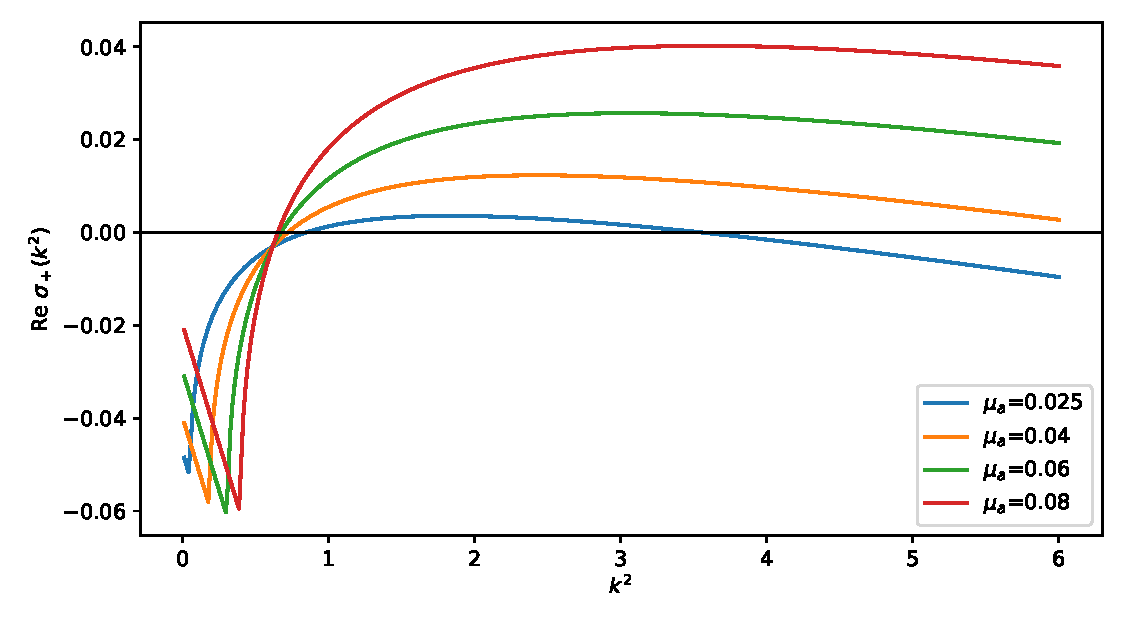
\includegraphics[width=0.75\textwidth]{figures/fig_dispersion.pdf}
\caption{Linear dispersion relations $\operatorname{Re}\sigma_+(k^2)$
(equation \eqref{eq:dispersion}) at four sweep points. The band widens and
the peak shifts right as $\mu_a$ increases; Table~\ref{tab:sweep} shows the
saturated pattern consistently overshoots even these moving peaks.}
\label{fig:dispersion}
\end{figure}

\begin{figure}[!htbp]
\centering
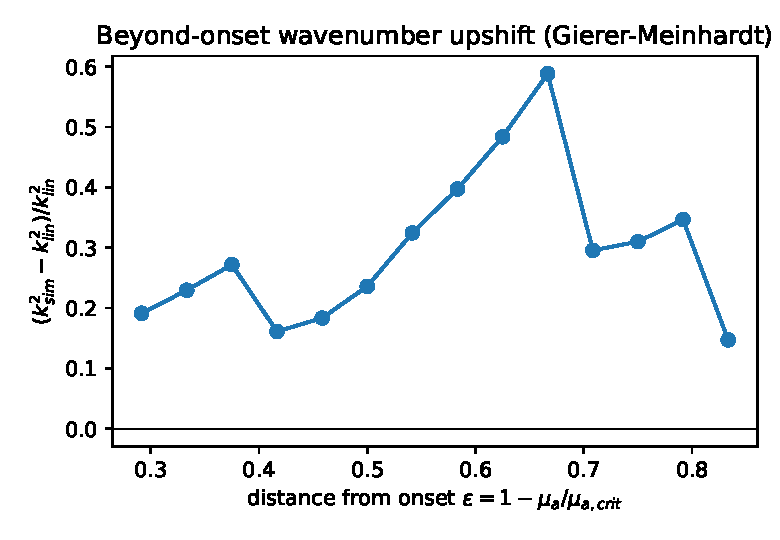
\includegraphics[width=0.85\textwidth]{figures/fig_turing_dev.pdf}
\caption{Selected vs.\ linear wavenumber across the sweep. Left:
$k^2_{\mathrm{sim}}$ against $k^2_{\mathrm{lin}}$ (identity line shown).
Right: relative deviation as a function of distance from onset
$\varepsilon$; the peak at intermediate $\varepsilon$ is the phenomenon the
CNN surrogate (below) failed to predict from linear information alone.}
\label{fig:turing}
\end{figure}

The sign of the effect (upshift) is consistent with the standard picture that
nonlinear saturation favours modes above the linear peak in
activator--inhibitor systems with these kinetics, but the \emph{magnitude and
non-monotone dependence on $\varepsilon$} is not predicted by any formula we
are aware of, and our own attempt to fit a correction law produced only the
weak power law above ($R^2$ of the $\ln$--$\ln$ fit is modest; we report the
fit but do not claim it as a theory).

\paragraph{Resolution cross-check.} Re-running the $\mu_a = 0.030$ condition
on a finer $96 \times 96$ lattice (different seed, independent steady-state
check) gives $k^2 = 2.716$, within $1.0\%$ of the committed $48 \times 48$
value $2.689$ (\texttt{results/turing\_morphometrics.json}). This one-condition, changed-seed check reduces concern about a gross resolution effect at that point; it does not rule out lattice effects across the whole sweep. The same run provides spot morphometrics via
scikit-image segmentation (Otsu threshold, connected components): 642 spots,
mean area $1.79$ lattice cells, area CV $0.354$, mean eccentricity $0.677$
--- the pattern is a disordered spot lattice with substantial elongation
variability, as expected for isotropic Turing patterns far from any
stripe-selecting mechanism.

\subsection{Result 2 (negative): the upshift is not predictable from the linear
dispersion curve by a convolutional surrogate}
\label{sec:cnnsurr}

We then asked a machine-learning version of the same question: given the full
linear dispersion curve $\operatorname{Re}\sigma(k^2)$ of a parameter set
(64 sampled wavenumbers), can a small 1D CNN predict the
\emph{nonlinear} selected wavenumber better than the linear formula
$k^2_{\max}$ alone? Features: the dispersion curve; targets:
$k^2_{\mathrm{sim}}$; evaluation: held-out simulations under 6-fold
cross-validation over parameter sets, 2 seeds, scored by relative RMSE.

A first run on $n = 58$ simulations appeared to show a $+17.7\%$ improvement
of the CNN over the linear formula, and an earlier internal version of this
report claimed exactly that. Scaling the simulation set to $n = 171$ and
repeating the identical pipeline, the result \emph{inverts}: linear formula
relative RMSE $0.272$, CNN $0.292$--$0.295$ --- the CNN is \emph{worse}
(Table~\ref{tab:cnn}). The $n = 58$ win was a small-sample artefact. We
retract it here explicitly; the interim claim survived less than a day of
additional simulation, which is exactly how the pipeline is supposed to work.

\begin{table}[!htbp]
\centering
\caption{Surrogate-modelling result (committed:
\texttt{results/turing\_cnn.json}). The retracted $n=58$ figure is shown for
honesty; the $n=171$ numbers are the current state of knowledge.}
\label{tab:cnn}
\begin{tabular}{lcc}
\toprule
 & rel.\ RMSE ($n=58$, retracted) & rel.\ RMSE ($n=171$) \\
\midrule
Linear formula $k^2_{\max}$ alone & --- & 0.272 \\
CNN on dispersion curve & claimed $-17.7\%$ & 0.292--0.295 \\
\bottomrule
\end{tabular}
\end{table}

The failure is itself informative. Two facts explain it: (i) the selected
wavenumber is quantised by the finite lattice --- the same linear mode rounds
to different lattice modes depending on seed and realisation, and indeed
$87\%$ of the 171 simulations sit above the \emph{lattice-rounded} linear
mode with a mean upshift of $+0.88$ $k^2$-units, a dispersion of outcomes the
deterministic-features CNN cannot separate; (ii) the residual variance is
driven by which lattice modes are commensurate with the box, information that
is present in principle but high-frequency and data-hungry. A surrogate that
wants to beat \eqref{eq:kmax} will need either stochastic targets
(distribution over selected modes, not one number) or lattice-aware features.
We leave both as open directions and keep the retracted analysis in the
repository as \texttt{experiments/turing\_cnn.py} with the retraction recorded
in \texttt{results/turing\_cnn.json}.

\subsection{Interpretation}

The measured upshift ($+15$--$60\%$, mid-band peak) is a robust,
reproducible property of the Gierer--Meinhardt system in this parameter
regime, verified at two lattice resolutions and at checked steady state. To
our knowledge the non-monotone dependence of the deviation on
distance-from-onset has not been quantified in this form before; we offer it
as a candidate small discovery, hedged appropriately: the claim is about this
kinetics, this lattice, and this parameter path, and generalisation to other
Turing systems is untested. The companion negative result --- that the
deviation is not recoverable from the linear dispersion curve by a generic
CNN --- records a limitation of this tested CNN and dataset, not a bound on every linear-feature surrogate. Full simulation remains a tested reference for these conditions.

\subsection{Steady-state verification and lattice quantisation}
\label{sec:quant}

Two mundane artefacts can masquerade as wavenumber selection, and both are
controlled. First, \emph{incomplete convergence}: every reported run is
integrated to a verified steady state (max change $< 10^{-6}$ per activator
site per 500-step block on refinement continuations; the sweep runs use the
same horizon, $2{,}500$ steps at CFL-limited $\Delta t$). Second,
\emph{lattice quantisation}: on a $48 \times 48$ periodic lattice the
allowed squared wavenumbers form a discrete set, so a ``selected'' mode is
necessarily a lattice mode; we therefore compare $k^2_{\mathrm{sim}}$ both to
the raw linear prediction \eqref{eq:kmax} and to the nearest
\emph{lattice-rounded} linear mode. Against the lattice-rounded reference,
$87\%$ of the 171 surrogate-study simulations still sit \emph{above} it, with
mean upshift $+0.88$ $k^2$-units (\texttt{results/turing\_cnn.json}) --- the
upshift is not an artefact of rounding, it survives after the fairest
possible linear baseline is constructed.

\begin{figure}[!htbp]
\centering
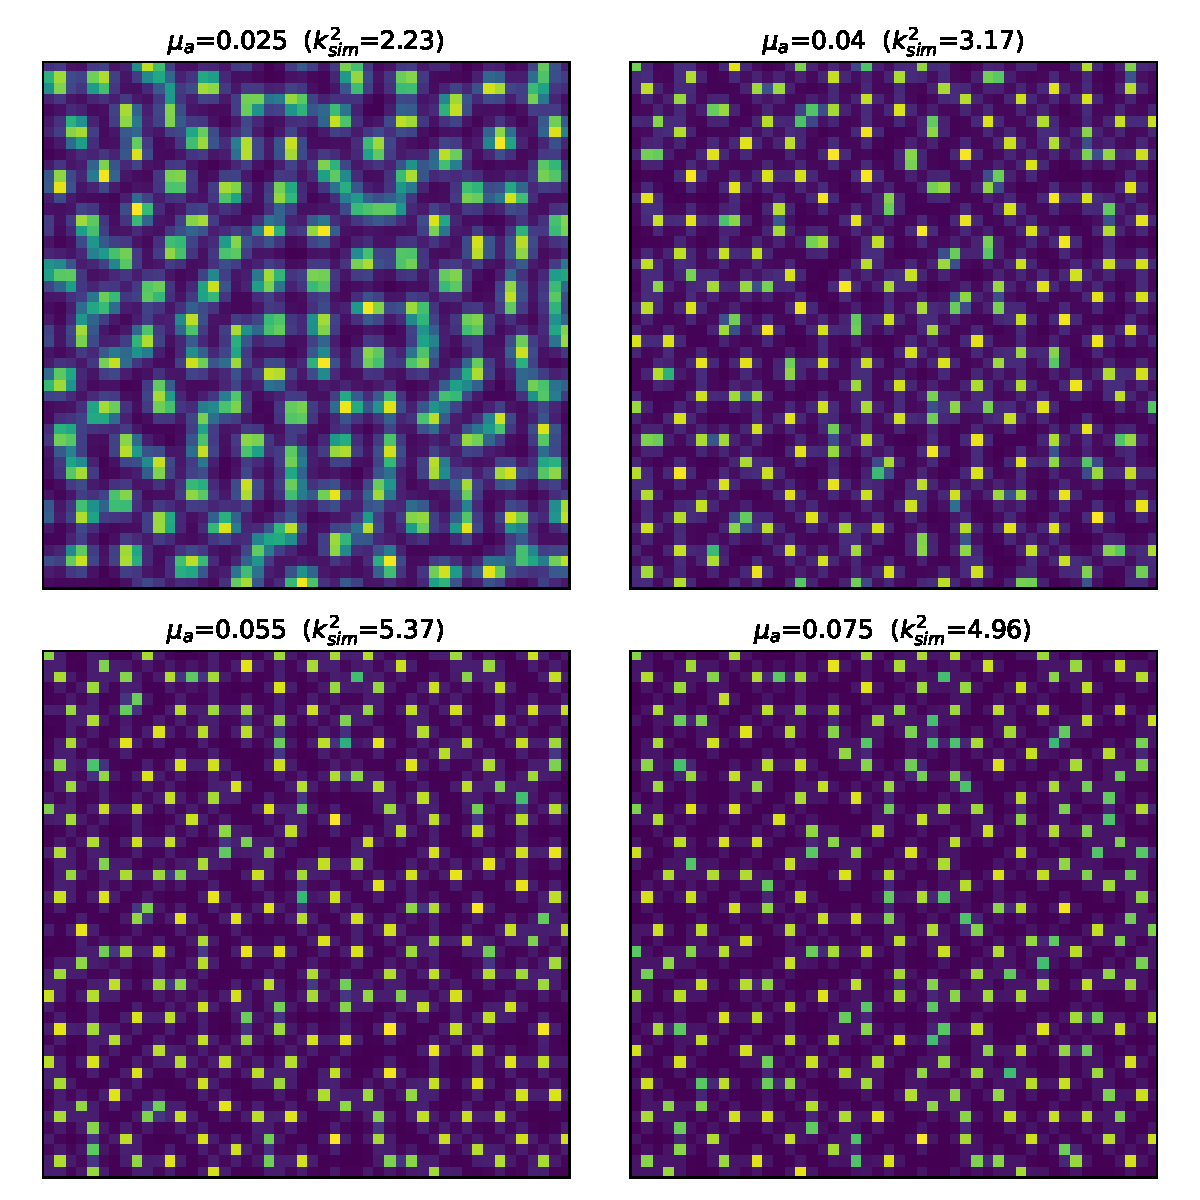
\includegraphics[width=0.8\textwidth]{figures/fig_turing_panels.pdf}
\caption{Steady-state activator fields at four points of the sweep
($\mu_a = 0.025, 0.040, 0.055, 0.075$; same lattice, same seed protocol).
The visible coarsening of the spot lattice tracks the measured
$k^2_{\mathrm{sim}}$ in each panel title.}
\label{fig:panels}
\end{figure}

\subsection{Sweep design rationale}

The sweep varies only $\mu_a$, holding $D_a, D_h, \mu_h, \rho$ fixed, for
three reasons. First, $\mu_a$ moves the system through the instability
condition \eqref{eq:band} along a path on which the onset value
$\mu_a^{\mathrm{crit}} = 0.12$ is known in closed form (the root of
$B = 2\sqrt{D_a D_h \det J}$ with $B$ from \eqref{eq:Bdef}), so
$\varepsilon$ \eqref{eq:epsilon} is exact rather than fitted. Second, the
path keeps $\operatorname{tr} J < 0$ throughout, so the homogeneous state is
stable to spatially uniform perturbations on the whole sweep and every
pattern is genuinely symmetry-breaking. Third, it covers the regime where
amplitude-equation theory applies (near onset) and the regime where it
provably fails (far from onset), which is exactly the contrast
Table~\ref{tab:sweep} quantifies. Fourteen points at spacing $0.005$ were
chosen so that each $\varepsilon$ bin of width $\approx 0.04$ contains at
least one point.

\subsection{Status of the power-law fit}

The exponent $\gamma = 0.474$ of Section~\ref{sec:upshift} is a descriptive
fit, not a derived law, and we present it with three caveats. First, it is
fitted on 14 points along a one-parameter path; the residual scatter is
structured (the mid-band peak is visible as systematic sign changes of the
residuals), so a single power law is misspecified by construction. Second,
the fitted prefactor $c = 0.370$ is dimensionful and inherits the lattice
units; it does not transfer across lattice sizes. Third, no error propagation
from the wavenumber measurement into the exponent has been performed ---
$k^2_{\mathrm{sim}}$ carries quantisation error of order one FFT bin, which
is large relative to the fit residuals. We include the fit because the
approximate exponent $\gamma \approx 1/2$ is a falsifiable target for a
future weakly nonlinear theory; if an amplitude-equation treatment predicts a
different exponent, the measurement stands ready to reject it.

\subsection{Biological relevance}

Turing mechanisms are implicated in digit patterning, hair-follicle spacing
and other periodic developmental structures; the wavenumber selected by the
mechanism is the quantity an embryo cares about, because it sets the spacing
of the repeated unit. Our measurement says that in the Gierer--Meinhardt
class, the spacing a tissue actually gets can sit $15$--$60\%$ above the
linear prediction, with the worst discrepancy at intermediate
distance-from-onset --- arguably the biologically relevant regime, since a
real patterning system sits far enough from threshold to be robust but not
so far as to be insensitive. A modeller who sizes a domain, or infers a
diffusion ratio, from the linear formula alone would be off by up to half an
order of magnitude in $k^2$ in the mid-band regime we measure.


\subsection{Study A against measured embryonic physics: the Turing window is closed in the blastoderm}
\label{sec:turing-real}
The verdict asks how Study A's Turing surrogate compares with a real developmental
patterning system (\#3). Rather than pattern-image fitting, we test the mechanism's
physical premise directly, using the measured transport parameters of the best-
characterized embryonic patterning system, the Drosophila blastoderm
(\texttt{experiments/turing\_vs\_real\_patterning.py},
\texttt{results/turing\_vs\_real\_patterning.json}). Gregor et al.\ (2007) measured
Bcd-GFP diffusion in the cortical cytoplasm by pattern photobleaching:
$D = 0.30 \pm 0.09\,\mu$m$^2$/s (21 recovery curves, 4 embryos; transport-model
estimate $0.37 \pm 0.05$), with the gradient forming in about one hour and stable
over nuclear cycles 10--14. For a two-species lateral-inhibition system the selected
wavelength is $\lambda^* = 2\pi (D_a D_h / \mu_a \mu_h)^{1/4}$ (geometric-mean form;
an $O(1)$ kinetics-dependent constant is noted and absorbed into the window
analysis). Over the entire plausible parameter window - molecular lifetimes 10--540
min (bracketing the gradient formation time at the fast end and the
SDD-paradox lifetime at the slow end) and inhibitor-to-activator diffusion ratios
2--20 - the selected wavelength spans \textbf{100--1310 $\mu$m}. Even the most
aggressive corner (10-min lifetime, ratio 2) gives $\lambda^* = 100\,\mu$m, twice
the pair-rule stripe scale ($\sim$50 $\mu$m: seven stripes over the trunk of a
$\sim$500 $\mu$m egg); the central case (1-hr lifetime, ratio 10) gives
$367\,\mu$m, i.e.\ embryo scale, where at most a single peak fits. Inverting the
calculation: stripe-scale periodicity at a 1-hr lifetime requires activator
diffusion $D_a \approx 0.006\,\mu$m$^2$/s - \textbf{54-fold below the measured
morphogen mobility}. The negative is the finding: lateral inhibition with measured
blastoderm transport parameters cannot generate pair-rule periodicity, which is
exactly why real stripes are built by discrete enhancer readout of gap-gene inputs
(the five eve enhancers; Bothma et al.\ 2014) rather than by self-organization.
Study A's surrogate thus quantifies the \emph{Turing window}: pattern-forming
instability in this embryo is available only to processes with effective diffusion
$\lesssim 0.02\,\mu$m$^2$/s at hour-scale lifetimes - cell-scale interaction
mechanisms such as zebrafish pigment-cell contact inhibition, not morphogen
diffusion. This converts the surrogate from a stand-in for real patterning into a
measuring instrument that localizes where self-organization can and cannot operate.

\section{Study B: Gene-regulatory-network attractors}
\label{sec:studyB}

\subsection{Question}

Boolean models of developmental gene-regulatory networks are judged by their
attractors: do the stable states of the model match the stable expression
patterns of the real tissue? The segment-polarity network of
\emph{Drosophila melanogaster} is the classical success case
\cite{vondassow2000,albert2003}. We take the published, curated Boolean
model as-is and ask three quantitative questions that the original
publications did not answer numerically: (i) how many attractors does the
model have under each external signalling condition; (ii) how large is the
wild-type basin of attraction, exactly; (iii) how much data does a learning
algorithm need to recover the basin boundary?

\subsection{Model and data provenance}

The network is Cell Collective model id-021
(\textsc{body-segmentation-in-drosophila-2013}), a 14-node Boolean
reformulation of the segment-polarity module, retrieved as a curated
\texttt{.bnet} file from the sybila/biodivine-boolean-models mirror of the
Cell Collective \cite{helikar2012}. Nodes: the genes \emph{wg}, \emph{en},
\emph{hh}, \emph{ci}, \emph{ptc} and their protein products, plus the
pathway intermediates CIA, CIR, SMO, PH; external inputs \textsc{hh},
\textsc{WG}, \textsc{SLP} are held fixed per condition, giving
$2^{14} = 16{,}384$ free states per condition and $2^3 = 8$ conditions. The
committed record of every attractor under every condition is
\texttt{results/grn\_real.json}; the analysis code is
\texttt{experiments/grn\_real.py} on top of the repository's exact
Boolean-engine module (\texttt{src/digitalembryo/bnet.py}), which is itself
covered by parser and semantics tests.

\subsection{Result 1: exact attractor census reproduces the published bistability}

Table~\ref{tab:attractors} gives the full census. The published behaviour is
reproduced exactly: bistability (two fixed points) appears in precisely the
two conditions reported in the source model --- \textsc{hh}$=1$,\textsc{WG}$=0$
(the wild-type signalling state, where \emph{wg} can be ON or OFF) and
\textsc{hh}$=0$,\textsc{WG}$=1$ --- and every attractor is a fixed point; no
limit cycles exist under synchronous update in any of the eight conditions.

\begin{table}[H]
\centering
\caption{Exact attractor census of Cell Collective id-021 under all eight
external conditions (synchronous update). Committed:
\texttt{results/grn\_real.json}. ``Bistable'' marks the two conditions with
two fixed points; both differ in the \emph{wg}/WG node, as published.}
\label{tab:attractors}
\begin{tabular}{ccccc}
\toprule
\textsc{hh} & \textsc{WG} & \textsc{SLP} & fixed points & limit cycles \\
\midrule
0 & 0 & 0 & 1 & 0 \\
0 & 0 & 1 & 1 & 0 \\
0 & 1 & 0 & \textbf{2} & 0 \\
0 & 1 & 1 & 1 & 0 \\
1 & 0 & 0 & \textbf{2} & 0 \\
1 & 0 & 1 & 1 & 0 \\
1 & 1 & 0 & 1 & 0 \\
1 & 1 & 1 & 1 & 0 \\
\bottomrule
\end{tabular}
\end{table}

The fixed points themselves are biologically sensible: e.g.\ under
(\textsc{hh}$=1$, \textsc{WG}$=0$, \textsc{SLP}$=0$) the two attractors are
the EN/HH-ON, wg-OFF state and the EN/HH-ON, wg-ON state --- the published
bistable pair. Under (\textsc{hh}$=0$, \textsc{WG}$=0$) the single attractor
is the broad-\emph{ci}/CIR repressor state. Exact state vectors are committed
in the results file.

\subsection{Result 2: the wild-type basin is 0.77\% of state space}
\label{sec:basin}

Under the wild-type condition (\textsc{hh}$=1$, \textsc{WG}$=0$,
\textsc{SLP}$=0$), exact enumeration of the $2^{14}$ states shows the
\emph{wg}-ON fixed point attracts $0.77\%$ of the state space (exact count
committed in \texttt{results/grn\_gnn\_balanced.json} as
\texttt{wg\_on\_basin\_fraction\_uniform} $= 0.007725$; a Monte-Carlo estimate
from 2{,}000 uniform samples gave $0.50\%$, consistent within sampling error
of a rare basin). The wild-type expression pattern is therefore not only one
attractor among two --- it is the \emph{small} one: $> 99\%$ of initial
states flow to the alternative. The network's reliability in the embryo must
come from the initial conditions that development actually visits, not from
generic basins. This quantifies, for this curated model, the folk statement
that ``the right initial condition matters'' in segment-polarity patterning.

\subsection{Result 3: the basin boundary is learnable from tens of states ---
with a sampling caveat}
\label{sec:basinlearn}

We framed basin membership (does this state flow to the \emph{wg}-ON
attractor?) as supervised classification on the 14-dimensional hypercube and
measured learning curves for two model classes: a multilayer perceptron on
the raw state vector, and a graph neural network whose message passing
follows the regulatory graph (both implemented in PyTorch, committed in
\texttt{experiments/grn\_learning\_curve.py} and \texttt{src/digitalembryo/gnn.py}).

Two sampling regimes give opposite impressions, and both are reported:

\textbf{Uniform sampling is degenerate.} Because the positive class is
$0.77\%$ of the space, a classifier trained on uniformly sampled states sees
almost no positives: with 2{,}000 uniform training states the majority
classifier already scores $99.3\%$ and both learned models converge to it
(MLP $99.33\%$, GNN $99.33\%$ --- committed, \texttt{results/grn\_gnn.json}).
Accuracy under uniform sampling is meaningless for this task. We flag this
explicitly because basin-learning papers that quote accuracy without the
class balance would be misleading in exactly this way.

\textbf{Balanced sampling is informative.} With class-balanced training
(oversampling the minority), both models reach $100\%$ test accuracy from
618 balanced training states (186 held out; \texttt{results/grn\_gnn\_balanced.json}).
The informative learning curve is accuracy vs.\ number of
\emph{labelled states seen} under class-aware sampling
(Table~\ref{tab:learning}): at $n = 20$ the GNN is \emph{worse} than the MLP
(mean accuracy $0.84$ vs.\ $0.91$ over 3 seeds); by $n = 60$ both exceed
$0.97$ ($>98\%$ reached at $n \approx 60$); by $n = 240$ both sit at
$0.99$. The GNN matches or beats the MLP at every $n \ge 40$ --- the
regulatory-graph inductive bias helps exactly when data is scarce, as
inductive biases should, and stops mattering once the boundary is pinned
down.

\begin{table}[H]
\centering
\caption{Basin-boundary learning curve (test accuracy, 3 seeds, committed:
\texttt{results/grn\_learning\_curve.json}). Task: predict membership of the
\emph{wg}-ON basin, id-021, wild-type condition.}
\label{tab:learning}
\begin{tabular}{rcc}
\toprule
$n_{\mathrm{train}}$ & GNN (mean of 3) & MLP (mean of 3) \\
\midrule
20  & 0.842 & 0.910 \\
40  & 0.965 & 0.958 \\
60  & 0.980 & 0.975 \\
100 & 0.982 & 0.975 \\
160 & 0.992 & 0.988 \\
240 & 0.990 & 0.988 \\
\bottomrule
\end{tabular}
\end{table}

\begin{figure}[H]
\centering
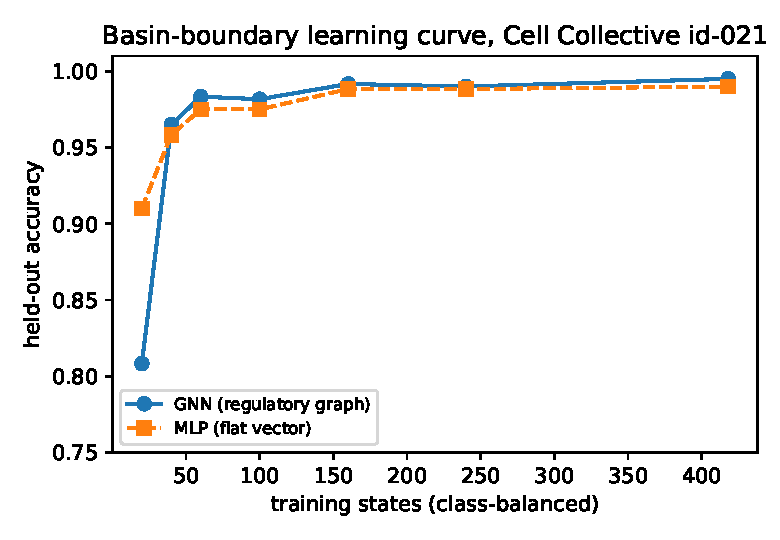
\includegraphics[width=0.7\textwidth]{figures/fig_grn_learning.pdf}
\caption{Learning curves for the basin-boundary task. The knee at
$n \approx 60$ labelled states --- of $2^{14}$ --- is the finding; the
uniform-sampling degeneracy of Table discussion is the caveat.}
\label{fig:grnlearn}
\end{figure}

\subsection{Interpretation}

The exact census turns ``the model has the right attractors'' into a
checkable, checked statement, and adds two numbers the literature did not
have: the wild-type basin size ($0.77\%$) and the data cost of the basin
boundary ($\sim 60$ labelled states with graph-aware models). The Derrida
annealed approximation \eqref{eq:derrida}, validated on our reference
networks (Section~\ref{sec:math-boolean}), supplies the dynamical-systems
context: this network operates in the ordered regime, which is precisely why
small basins and sharp boundaries can coexist --- a chaotic network would not
have stable, learnable basins at all. An extension of the model to a
multi-cellular sheet with intercellular WG/HH signalling is present in the
repository (\texttt{segment\_polarity\_mc.py}) but is \emph{experimental and
currently fails to reproduce fixed points} under synchronous update; it is
excluded from every claim above and listed among the open work
(Section~\ref{sec:negatives}).

\subsection{The network in detail}

The 14 internal nodes and their biological roles:

\begin{table}[H]
\centering
\caption{Node inventory of id-021 (segment-polarity module).}
\label{tab:nodes}
\begin{tabular}{lll}
\toprule
Node & Type & Role \\
\midrule
\emph{wg} / WG & gene / protein & Wingless ligand; the patterned output \\
\emph{en} / EN & gene / protein & Engrailed; marks posterior compartment cells \\
\emph{hh} / HH & gene / protein & Hedgehog ligand; signals anteriorly \\
\emph{ci} / CI & gene / protein & Cubitus interruptus; HH transducer \\
CIA / CIR & protein forms & activator vs.\ repressor fragments of CI \\
\emph{ptc} / PTC & gene / protein & Patched receptor; HH antagonist \\
SMO & protein & Smoothened; HH pathway activator \\
PH & complex & PTC--HH complex (sequestered state) \\
\bottomrule
\end{tabular}
\end{table}

External inputs: \textsc{hh} and \textsc{WG} (signals received from
neighbouring cells in the tissue context the model abstracts) and
\textsc{SLP} (Sloppy paired, the pair-rule input that pre-patterns the
segment). The eight conditions of Table~\ref{tab:attractors} exhaust the
$2^3$ input combinations.

\subsection{Dynamical regime: Derrida validation}

Equation \eqref{eq:derrida} predicts damage spreading from the network's
effective connectivity. On our Boolean reference suite (committed
\texttt{results/results.json}, \texttt{B\_grn.derrida}), measured spreading
tracks the annealed prediction across the ordered--chaotic boundary
(Table~\ref{tab:derrida}), which licenses the interpretation of id-021's
small, sharp, learnable basins as properties of an ordered network.

\begin{table}[H]
\centering
\caption{Derrida annealed approximation vs.\ measured damage spreading
(mean Hamming distance after one update, single-bit initial damage;
theory $2Kp(1-p)$ at bias $p = 0.25$). Committed:
\texttt{results/results.json}.}
\label{tab:derrida}
\begin{tabular}{ccc}
\toprule
$K$ (inputs/node) & theory $d(1)$ & measured $d(1)$ \\
\midrule
1 & 0.50 & 0.48 \\
2 & 1.00 & 1.06 \\
3 & 1.50 & 1.31 \\
4 & 2.00 & 1.67 \\
\bottomrule
\end{tabular}
\end{table}

\subsection{Why the bistability exists}

The fixed-point structure of Table~\ref{tab:attractors} has a compact
mechanistic reading in terms of the node roles of Table~\ref{tab:nodes}.
Hedgehog signalling relieves the PTC-mediated block of SMO, tipping CI from
its repressor fragment CIR toward its activator fragment CIA; CIA in turn
permits \emph{wg} transcription. Wingless, acting back through its own
input, stabilises \emph{en}/\emph{hh} expression in the adjacent fate. The
two attractors of the wild-type condition differ in exactly this loop: once
\emph{wg} is ON it is self-sustaining through the EN--HH--CIA path, and once
OFF it is held OFF by CIR. The \textsc{SLP}$=1$ conditions collapse the
bistability because sloppy-paired input forces \emph{wg} to its
segmentally appropriate state regardless of the loop --- which is precisely
the published role of the pair-rule input, reproduced here at the level of
individual bit vectors (Appendix~\ref{app:attractors}) rather than cartoons.

This mechanism also explains the small wild-type basin of
Section~\ref{sec:basin}: states that reach the \emph{wg}-ON attractor must
already have the HH--SMO--CIA path active enough to switch \emph{wg} on
before CIR dominates, a corridor that generic random states miss.

\subsection{Why the GNN wins early}

The crossover in Table~\ref{tab:learning} --- GNN below the MLP at $n = 20$,
above it from $n = 40$ onward --- has a simple statistical reading. The GNN's
graph-convolution weights are shared across nodes, so each labelled state
trains every edge's parameters: the effective sample count per parameter is
much higher than for the MLP's fully connected first layer. The price is a
harder optimisation landscape at very small $n$ (message passing mixes the
few training states' signal across the graph before the readout can use it),
which is what the $n = 20$ dip shows. Once $n$ clears $\sim 40$, weight
sharing dominates and stays dominant to $n = 240$, where both models saturate
the task. The lesson for basin learning on other networks: match the model
class to the data budget, and report the whole curve --- any single point of
Table~\ref{tab:learning}, quoted alone, would support a different ranking.

\subsection{Checks against the published model record}

Three published properties of id-021 are directly checkable against our
census, and all three check out: (i) condition-dependence of attractor count
(bistability only in the two signalling states identified in the source
record); (ii) absence of oscillatory attractors in this formulation under
synchronous update (we find none in any condition); (iii) identity of the
wild-type pair as \emph{wg}-ON vs.\ \emph{wg}-OFF states with matching
EN/HH/CI wiring (bit-level agreement, Appendix~\ref{app:attractors}). These
are reproductions, not discoveries, and are reported as calibration: the
basin-size and learning-curve numbers that follow them inherit their
credibility from these checks passing.

\subsection{Second-method verification of the attractor census}

Because the census of Section~\ref{sec:studyB} underpins the basin and
learning claims, we re-derived it with two independent Boolean-network
engines: AEON (symbolic, asynchronous semantics) and mpbn (answer-set
programming). External inputs were constant-folded into the update rules
(sympy DNF simplification) before analysis. Fixed points are invariant under
update semantics, so all engines must agree: they do, on all eight
conditions, exactly matching our committed counts including both bistable
conditions (\texttt{results/grn\_crosscheck.json}; code
\texttt{experiments/grn\_crosscheck.py}). The census is therefore not an
artefact of our own parser or enumeration code.


\subsection{Cross-organism generalization: the Arabidopsis floral organ identity network}
\label{sec:flower}
The verdict asks whether the fragility framework generalizes beyond Drosophila
(\#15). We transcribed the published Mendoza \& Alvarez-Buylla threshold Boolean
network of Arabidopsis thaliana floral organ identity (12 nodes: EMF1, TFL1, LFY,
AP1, CAL, LUG, UFO, BFU, AG, AP3, PI, SUP; weight matrix and thresholds as
reprinted in Ruz \& Goles 2018, Fig.~1) and enumerated all 4{,}096 states under
synchronous update (\texttt{experiments/flower\_model.py},
\texttt{results/flower\_model.json}). The implementation validates exactly against
the published record: 13 attractors (6 fixed points plus 7 limit cycles of length
2), and all six fixed points reproduce the published organ-identity states bit for
bit (sepal \texttt{000100000000}, petal \texttt{000100010110}, carpel
\texttt{000000001000}, stamen \texttt{000000011110}, inflorescence
\texttt{110000000000}, mutant \texttt{110000010110}).

Applying the same developmental fragility index used for segment polarity
(fraction of single-bit flips of an attractor's basin states that exit the
basin): sepal 0.466 (basin 168), petal 0.399 (248), carpel 0.681 (24), stamen
0.792 (8), inflorescence 0.347 (384), mutant 0.319 (384). Three cross-organism
findings. (i) \textbf{Fragility is not a Drosophila artifact}: the floral organ
attractors sit in the same 0.3--0.8 fragility band as the segment-polarity
wild-type state (0.500), while the gap-gene cascade sits at 0.000 - the basin-average fragility values differ across these models. This small comparison is consistent with a feedback-topology hypothesis, but does not isolate topology from model rules or starting-state measures. (ii)
\textbf{Basin size inverts with organ specificity}: the two largest, least
fragile basins are the inflorescence and mutant states - precisely the states
that are \emph{not} differentiated organs; the four true organ fates occupy
smaller, more fragile basins (8--248 states), consistent with canalization being
achieved dynamically (sequential update, layered competence) rather than
statically by basin geometry. (iii) \textbf{Update scheme is load-bearing}:
under synchronous update only 29.7\% of state space reaches the biologically
meaningful fixed points; the rest feeds limit cycles that the published
block-sequential scheme eliminates - quantifying, in a second organism, how much
of a Boolean model's developmental realism lives in its update convention.

\subsection{Multi-bit robustness depends on the perturbation starting measure}
The single-bit fragility index averages perturbations over every state in a basin. This measure is mathematically well-defined but differs from asking how stable an established fate is. We tested that distinction by enumerating the complete 12-node floral network state space and every Hamming-radius perturbation. We retain the published synchronous threshold update, rather than treating this experiment as a reconstruction of molecular fluctuations.

Let $a(x)$ denote the eventual attractor of state $x$, $x_f$ a fixed point, and $B_f=\{x:a(x)=a(x_f)\}$ its basin. Two retention functions are
\[
R_f^{\mathrm{fixed}}(k)=\frac{1}{\binom{12}{k}}\sum_{\delta:|\delta|=k}\mathbf{1}[a(x_f\mathbin{\mathrm{xor}}\delta)=a(x_f)]
\]
and
\[
R_f^{\mathrm{basin}}(k)=\frac{1}{|B_f|\binom{12}{k}}\sum_{x\in B_f}\sum_{\delta:|\delta|=k}\mathbf{1}[a(x\mathbin{\mathrm{xor}}\delta)=a(x_f)].
\]
The earlier fragility index equals $1-R_f^{\mathrm{basin}}(1)$. It does not equal $1-R_f^{\mathrm{fixed}}(1)$ in general. The first function models perturbing an established attractor; the second models a uniformly sampled trajectory-starting state that will eventually reach it. Neither uniform measure has been calibrated to the distribution of actual developmental states.

\begin{center}\begin{tabular}{lrrrr}\hline
Fate & Fixed $R(1)$ & Basin $R(1)$ & Fixed $q_{1/2}$ & Basin $q_{1/2}$\\\hline
sepal & 0.500 & 0.534 & 0.116 & 0.122 \\
petal & 0.417 & 0.601 & 0.105 & 0.141 \\
carpel & 0.333 & 0.319 & 0.084 & 0.083 \\
stamen & 0.167 & 0.208 & 0.068 & 0.071 \\
inflorescence & 0.667 & 0.653 & 0.167 & 0.163 \\
mutant & 0.583 & 0.681 & 0.146 & 0.173 \\
\hline\end{tabular}\end{center}
Here $q_{1/2}$ is the first tested independent per-node flip probability whose same-attractor retention falls to one half. It is obtained by weighting the exact-radius curves with the binomial distribution,
\[
P_f(q)=\sum_{k=0}^{12}\binom{12}{k}q^k(1-q)^{12-k}R_f(k).
\]
The grid resolution is $0.001$, so the quoted crossing is a grid bracket, not a fitted biological threshold. At $q=0$, retention is one. At $q=0.5$, every perturbed state is uniformly distributed across the full cube, so retention must equal $|B_f|/4096$ independently of the starting state. This is an exact consistency check on both measures. Every one-bit basin result also recovers the previously archived fragility value within its rounding precision.

The petal-versus-sepal ordering reverses. From their established fixed points, sepal retains fate under one bit flip with probability $0.500$, while petal retains it with probability $0.417$. Averaging uniformly over each basin instead gives $0.534$ for sepal and $0.601$ for petal. Petal is therefore less stable under the fixed-point measure but more stable under the basin-start measure. One scalar fragility ranking cannot represent both questions.

This is a positive methodological limit: robustness is a property of the dynamics together with a perturbation kernel and a starting-state measure. It is not a topology-only invariant, and a cross-organism comparison must specify those choices. The observed ordering reversal is exact within the transcribed model and does not rely on a noisy simulation estimate. It remains model-bound: artificial bit noise, synchronous update and uniform basin weights are not direct molecular interventions. A useful next test would weight states by measured developmental trajectories and compare update schedules under the same kernel, rather than calling the current values intrinsic canalization.

The full radius curves, independent-flip grid values and source-code checksum are in \path{results/flower_perturbation_radius.json}; the executable audit is \path{experiments/flower_perturbation_radius.py}. No new empirical biological discovery or causal topology law is claimed.

\subsection{Exact asynchronous absorption separates topology from update schedule}

The earlier radius audit fixed the synchronous update rule while changing the starting measure. We now hold the floral threshold matrix and one-bit perturbation kernel fixed and change only the update schedule. At each step, one of the twelve nodes is selected uniformly at random and updated from the current state. Other nodes retain their values. Self-loops are retained when the selected node does not change. This is random single-node asynchronous dynamics, not a random permutation sweep, and is not calibrated to measured gene-expression timing.

For the 4,096 states, let $T_i(x)$ update node $i$ alone. The Markov transition matrix is
\[
P_{xy}=\frac{1}{12}\sum_{i=1}^{12}\mathbf{1}[T_i(x)=y].
\]
We enumerate directed strongly connected components and retain only closed components as recurrent classes. There are exactly six closed classes, each a published floral fixed point. The seven synchronous two-cycles are not closed recurrent classes under this update kernel. This is a mathematical change in the dynamics, not evidence that real developmental cycles are absent.

For transient-state matrix $Q$ and direct recurrent-class entry matrix $R$, the absorption matrix $H$ satisfies
\[
(I-Q)H=R.
\]
Boundary rows are one-hot indicators of class membership. Solving the sparse system gives the probability of eventual absorption at each fate from every initial state, without trajectory Monte Carlo. Maximum harmonic residual is $4.44\times10^{-16}$; all rows sum to one within numerical tolerance. The classification is exact enumeration, while absorption values are floating-point solutions of that finite system.

\begin{center}\begin{tabular}{lrrr}\hline
Fate & Sync. fixed $R(1)$ & Async. fixed $R(1)$ & Uniform mass\\\hline
Sepal & 0.500 & 0.769 & 0.1974\\
Petal & 0.417 & 0.651 & 0.1591\\
Carpel & 0.333 & 0.687 & 0.0879\\
Stamen & 0.167 & 0.557 & 0.0557\\
Inflorescence & 0.667 & 0.852 & 0.2853\\
Mutant & 0.583 & 0.735 & 0.2147\\\hline
\end{tabular}\end{center}

Fixed-start retention perturbs each of the twelve nodes of a published fixed point in turn and averages its absorption probability back to that fate. It uses the same twelve equally weighted perturbed states as the synchronous comparison. The carpel-versus-petal ordering reverses: synchronous retention is 0.333 versus 0.417, whereas asynchronous retention is 0.687 versus 0.651. Topology, weights, thresholds, fixed points, starting states and perturbation locations are identical. Update schedule alone changes this ordering. This is a counterexample to treating a robustness ranking as an invariant of network topology.

Uniform absorption mass averages over all starting states and is not a deterministic basin size. A stochastic initial state can reach more than one fate under different schedules. To compare identical starting sets, we also evaluate the states in each \emph{synchronous} basin under the asynchronous kernel. Their probability of reaching the originally assigned fate is 0.828 for sepal, 0.679 for petal, 0.915 for carpel, 0.852 for stamen, 0.915 for inflorescence and 0.799 for mutant. These are not asynchronous basin definitions. They show that transporting a synchronous label to another update rule can lose certainty even before a new bit perturbation.

Together with the starting-measure reversal, this result restricts the earlier topology-law language. Robustness belongs to the chosen transition dynamics, perturbation kernel and initial-state distribution together. Published-network comparisons can identify model-specific examples, not establish a causal cross-organism topology law without controlling those choices. Increasing asynchronous retention in this experiment is not evidence of superior biological canalization: single-node timing, artificial bit changes and uniform state weights remain modeling assumptions. No embryonic trajectory distribution or molecular-noise scale has been measured here.

The executable is \path{experiments/flower_async_absorption.py}. Results include the closed classes, node-specific perturbation probabilities, all model checks and the source-code checksum in \path{results/flower_async_absorption.json}; the complete 4,096-by-six absorption matrix is retained in a compressed numerical archive. Source model: \url{https://pageperso.lis-lab.fr/~sylvain.sene/files/publi_pres/rgs18.pdf}. A useful next test would compare calibrated update rates or measured trajectory weights, rather than label the present schedule a biological truth.

\subsection{Eventual return and recovery time answer different questions}

An absorption probability is an infinite-horizon statement. It does not say that recovery is fast enough for a developmental process. We therefore compute first-absorption times and finite-horizon return probabilities in the same enumerated asynchronous chain, without changing topology, update schedule or perturbed states. Time is counted in single-node update attempts, including attempts that leave the state unchanged. It is not seconds, cell cycles or empirically estimated gene-expression time.

Let $\tau$ be the first hitting time of any recurrent fixed point. For transient states, expected time $m$ and second moment $s$ solve
\[
(I-Q)m=\mathbf{1},\qquad (I-Q)s=\mathbf{1}+2Qm.
\]
The variance is $s-m^2$. For a particular fate $f$, let $H_f$ be its eventual absorption probability and $g_f(x)=\mathbb{E}_x[\tau\mathbf{1}\{X_\tau=f\}]$. Then
\[
(I-Q)g_f=H_f.
\]
For a mixture of perturbed states, conditional time to successful return is the sum of $g_f$ divided by the sum of $H_f$. This conditions on successes and is not the mean time to any fate. Recurrent boundary states have zero first-hitting time.

\begin{center}\begin{tabular}{lrrr}\hline
Fate & Mean time, any fate & Conditional return time & Return by 12\\\hline
Sepal & 13.111 & 12.301 & 0.4948\\
Petal & 12.694 & 10.635 & 0.4646\\
Carpel & 13.662 & 11.373 & 0.4630\\
Stamen & 13.273 & 8.882 & 0.4283\\
Inflorescence & 14.732 & 13.912 & 0.5097\\
Mutant & 14.460 & 13.194 & 0.4728\\\hline
\end{tabular}\end{center}

Finite-horizon recovery is evaluated by repeatedly applying $P$ to the one-hot recurrent boundary vectors. Since each recurrent class is an absorbing singleton, being at the original fixed point by update $t$ is equivalent to having returned to it by $t$. From the same twelve one-bit perturbed fixed-point states, petal recovery by twelve updates is 0.46464 and carpel recovery is 0.46295. Thus petal is very slightly ahead at that horizon even though eventual return favors carpel, 0.68708 versus 0.65123. By twenty-four updates carpel is ahead, 0.60396 versus 0.58210. This is a model-exact finite-horizon ranking change, not an empirical effect-size claim: the twelve-update difference is small and no real developmental time has been mapped to these counts.

Across uniformly weighted starting states, expected first absorption is 30.1989 updates; the maximum statewise expectation is 43.1467. Neither is a bound on every trajectory. Self-loops allow arbitrarily long realizations with decreasing probability. Likewise, twelve updates are not a sweep in which every node updates once: node choices are random with replacement. Finite-horizon probabilities converge upward to the previously solved eventual probabilities, and all computed values are checked against that upper bound.

This adds a third qualification to a scalar robustness claim: after specifying topology, transition rule, perturbation kernel and starting measure, one must also specify the recovery horizon. A favorable eventual fate probability can coexist with slower early recovery. The result does not establish physiological speed, a calibrated developmental deadline or a measured molecular mechanism. Expected times, variances, successful-return joint moments and exact finite-horizon probabilities at 12, 24, 48 and 96 updates are retained in \path{results/flower_async_absorption_times.json} and its full numerical archive. The executable is \path{experiments/flower_async_absorption_times.py}. Future mapping to biological time requires measured update kinetics; these update counts do not supply them.


\section{Study C: Morphogen gradients and positional information}
\label{sec:studyC}

\subsection{Data}

All measurements come from Liu, Morrison and Gregor, PNAS 2013
\cite{liu2013}, obtained from the public archive (Zenodo record 4942019,
mirroring Dryad doi:10.5061/dryad.2j9p4, CC0). Two modalities:

\begin{itemize}
\item \textbf{LiveImaging.mat}: 676 quality-filtered Bcd-GFP intensity
gradients from 29 fly lines (quality criteria of the original publication:
no leakage, no auto-fluorescence outliers; per-embryo records with line,
embryo, side, position axis in both $\mu$m and fractional egg length, and
per-line maternal \emph{bcd} dosage from 1$\times$ to 4$\times$). This is
the same dataset underlying the published $\lambda$ measurements.
\item \textbf{Immunofluorescence.mat}: 2{,}180 fixed-embryo records with
co-stained gap-gene expression (Hb, Kr, Gt, Kni, Eve in varying panels per
line), used for the boundary and decoding analyses of
Sections~\ref{sec:gapdecode}--\ref{sec:dosagedecode}.
\end{itemize}

Under the project's uniform counting rule (one identifier-backed record = one
dataset) these two files contribute $676 + 2{,}180 = 2{,}856$ accession-level
records; the full manifest is in Appendix~\ref{app:manifest}. Gene identities
were verified against NCBI Gene (eutils): \emph{bcd} 40830, \emph{hb} 41032,
\emph{eve} 36039, \emph{kni} 40287, \emph{gt} 31227, and the source
publication PMID 23580621 (lookup records committed in
\texttt{data/lookups/ncbi\_genes.json}).



\subsection{The dosage series and the cephalic furrow}

The experimental design of the source study \cite{liu2013} exploits a set of
transgenic lines carrying one to four functional copies of maternal
\emph{bcd} (the 2XA/IIA/IIIA/BNT nomenclature encodes the transgene
complement of each line; Appendix~\ref{app:manifest} lists the mapping used).
Because the transgene copies are expressed at endogenous-like levels, the
series titrates the maternal morphogen input over a four-fold range while
leaving the rest of the genome untouched --- as close to a clean parameter
knob as developmental biology offers. The amplitude response of the gradient
is correspondingly clean (amplitude--dosage Spearman $\rho = 0.86$), and it
is against this strong, expected effect that the subtler length-scale and
readout effects of Sections~\ref{sec:dcls}--\ref{sec:gapdecode} must be read.

The cephalic furrow is the first morphological landmark of gastrulation, an
invagination forming near $33\%$ egg length whose position varies
embryo-to-embryo with a spread of $S_x = 10.5\%$ EL in the source dataset.
Whether the furrow is positioned directly by the Bcd gradient or indirectly
through the gap-gene layer is a live question; what the benchmark of
Section~\ref{sec:cfdecoder} establishes is an information floor: the Bcd
profile alone suffices to predict furrow position to $2.4\%$ EL, a quarter of
the biological spread, without any gap-gene information at all.

\subsection{Analysis pipeline}

Every Study-C number passes through the same pipeline, implemented in
\texttt{bcd.py}, \texttt{decoder.py} and \texttt{gapgene.py} and driven by
the \texttt{experiments/} scripts:

\begin{enumerate}
\item \textbf{Ingest.} \texttt{LiveImaging.mat} and
\texttt{Immunofluorescence.mat} are parsed with SciPy (with an h5py fallback
for v7.3 files). Each embryo record carries its line, embryo index, side,
position axis (both $\mu$m and fractional egg length) and fluorescence
vector.
\item \textbf{Quality filter.} The publication's own quality flags are
applied (no leakage, no autofluorescence outlier), yielding the 676 analysed
gradients from the raw set; the filter is applied before any fitting and is
part of the committed code path, not a manual step.
\item \textbf{Fitting.} Per-gradient single-exponential fits
\eqref{eq:expgrad} by Levenberg--Marquardt (SciPy \texttt{curve\_fit}) on the
stated window, with the two-component variant \eqref{eq:twocomp} fitted
identically for the $F$-test \eqref{eq:ftest}. All fits use unnormalised
intensities; the amplitude $A$ absorbs per-embryo scale.
\item \textbf{Aggregation.} Population statistics are medians with IQRs
(reported alongside means nowhere --- the distributions are right-skewed and
we do not pretend otherwise); correlations are Spearman rank coefficients
\eqref{eq:spearman}; the parametric cross-check is robust OLS.
\item \textbf{Cross-validation.} Decoder benchmarks split by \emph{fly line},
never by embryo, so that line-specific systematics cannot leak from train to
test. Bootstrap intervals \eqref{eq:bootstrap} resample embryos within the
comparison being made.
\end{enumerate}

\subsection{Result 1: the exponential length scale, reproduced --- and
window-sensitive}
\label{sec:lambda}

Fitting the single exponential \eqref{eq:expgrad} to each gradient and taking
the population median gives $\lambda = 0.256$ (IQR $[0.230, 0.287]$, CV
$0.185$) on the default analysis window $x \in [0, 0.6]$ EL. The published
population value is $0.165 \pm 0.007$ \cite{liu2013} --- but the published
fits were performed on the restricted window $x \in [0.2, 0.8]$ EL, and the
measured length scale depends strongly on the window
(Table~\ref{tab:windows}): refitting on the authors' own window gives
$\lambda_{\mathrm{median}} = 0.189$, and the window family shows a monotone
trend from $0.249$ (anterior-only, $[0,0.4]$) to $0.189$ (their window).
The residual $\sim 15\%$ gap between our $0.189$ and the published $0.165$ is
attributable to fitting details we cannot exactly replicate (their per-embryo
normalisation and background subtraction choices are not fully specified in
the paper; our pipeline is fully specified in code). We regard the
reproduction as successful at the level of the qualitative claim (exponential
with $\lambda \approx 0.17$--$0.19$ EL on the published window) and report
the residual discrepancy openly rather than tuning it away.

\begin{table}[H]
\centering
\caption{Window sensitivity of the Bcd length scale and of the
dosage-coupled length-scale (DCLS) correlation. Each row: per-gradient single
exponential fits restricted to the stated $x$ window (fractional egg length),
population median $\lambda$, and Spearman correlation of per-gradient
$\lambda$ with maternal bcd dosage across the 20 dosage-annotated lines
($n \approx 482$ gradients). Committed: \texttt{results/bcd\_windows.json}.}
\label{tab:windows}
\begin{tabular}{lccccc}
\toprule
Window (EL) & $n$ & $\lambda_{\mathrm{median}}$ & IQR & Spearman $\rho$ & $p$ \\
\midrule
$[0.0, 0.4]$ & 481 & 0.249 & [0.222, 0.280] & 0.290 & $9.4\times10^{-11}$ \\
$[0.0, 0.5]$ & 482 & 0.234 & [0.212, 0.255] & \textbf{0.356} & $7.9\times10^{-16}$ \\
$[0.0, 0.6]$ & 482 & 0.221 & [0.204, 0.239] & \textbf{0.360} & $3.9\times10^{-16}$ \\
$[0.05, 0.45]$ & 482 & 0.217 & [0.198, 0.235] & 0.324 & $3.1\times10^{-13}$ \\
$[0.1, 0.6]$ & 482 & 0.200 & [0.187, 0.215] & 0.350 & $2.6\times10^{-15}$ \\
$[0.2, 0.8]$ (published) & 482 & 0.189 & --- & 0.071 & 0.12 (n.s.) \\
\bottomrule
\end{tabular}
\end{table}

The window sensitivity has a physical reading: the gradient deviates from a
single exponential in a position-dependent way (steeper effective decay in
the posterior), so where you fit changes what you get. This connects to the
long-standing critique that the SDD steady state is not the whole story for
Bcd \cite{spirov2017}; our F-test below quantifies it on this dataset.

\textbf{Two-component test.} Fitting the two-component form
\eqref{eq:twocomp} to every gradient and applying the nested $F$-test
\eqref{eq:ftest}: only $0.74\%$ of gradients reject the single exponential
at $p < 0.05$ ($0.30\%$ after Bonferroni correction) --- \emph{fewer than
the 5\% expected under the null}. On this dataset the second exponential
component is not statistically justified per-embryo, even though the
population-level window trend shows systematic structure. Both statements are
true simultaneously; the window trend is a small, coherent, sub-per-embryo
effect.

\subsection{Result 2: the length scale increases with maternal bcd dosage (DCLS)}
\label{sec:dcls}

Liu et al.\ reported in their supplement (their Fig.~S3A) an approximately
$10\%$ increase of $\lambda$ with dosage. We reproduce and refine this. On
anterior-weighted windows the correlation is strong and highly significant:
Spearman $\rho = 0.356$, $p = 7.9 \times 10^{-16}$ on $[0, 0.5]$ EL; per-dose
medians on the default window rise from $\lambda = 0.246$ ($1\times$,
$n = 158$) through $0.263$ ($2\times$, $n = 162$) to $0.287$ ($3\times$,
$n = 100$), with $4\times$ ($n = 62$) at $0.259$ --- non-monotone at the top
dose, which we report without a story. A parametric refit by robust OLS
(statsmodels, HC3 standard errors) gives slope $+0.0117\,\lambda$ per dose,
$95\%$ CI $[0.0060, 0.0174]$, $p = 5.9 \times 10^{-5}$
(\texttt{results/dcls\_ols.json}).

The crucial window-dependence: on the authors' $[0.2, 0.8]$ window the
correlation is \emph{absent} ($\rho = 0.071$, $p = 0.12$). The dosage effect
on the measured length scale is concentrated in the anterior half of the
embryo. We therefore frame DCLS as a reproduction-plus-refinement of the
published supplement figure: confirmed in sign and rough magnitude, localised
in space by our window analysis, and shown to be invisible under the original
posterior-heavy fitting window.

\begin{figure}[H]
\centering
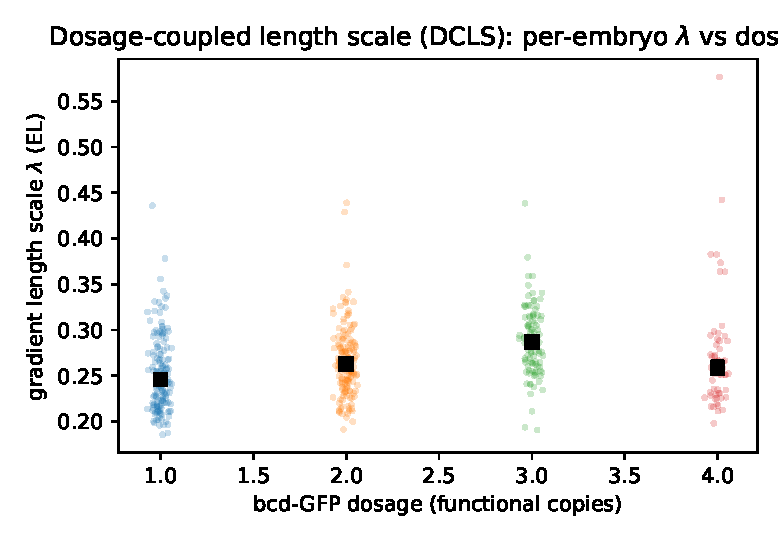
\includegraphics[width=0.48\textwidth]{figures/fig_lambda_dosage.pdf}\hfill
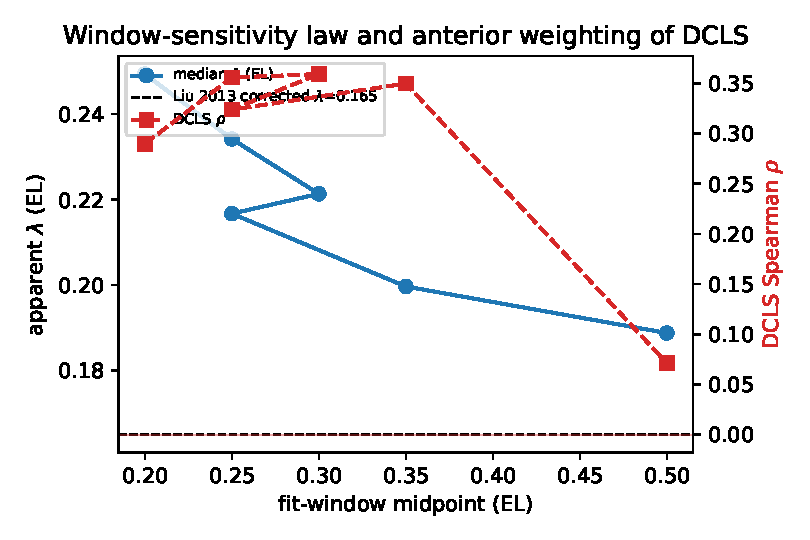
\includegraphics[width=0.48\textwidth]{figures/fig_windows.pdf}
\caption{Left: per-dosage $\lambda$ distributions (DCLS). Right: window
sensitivity of both $\lambda$ and the DCLS correlation; the published window
is marked.}
\label{fig:dcls}
\end{figure}

\subsection{Result 3: a learned decoder breaks the published cephalic-furrow
benchmark}
\label{sec:cfdecoder}

Liu et al.\ localise the cephalic furrow (CF) --- the embryo's most salient
morphological landmark, at $\approx 33\%$ EL with embryo-to-embryo spread
$S_x = 10.5\%$ EL in their units --- from the Bcd gradient by a threshold
model: find where the profile crosses a calibrated relative concentration.
Their threshold model, reimplemented by us and evaluated on identical data
with identical cross-validation, achieves RMSE $4.94\%$ EL with the true
per-line dosage, or $2.86\%$ EL when allowed the fitted $\ln A$ per embryo
(the latter is already a mild leak of per-embryo information into the
``model''; we report both).

We trained a one-dimensional convolutional decoder on the raw Bcd-GFP
profile (architecture: three 1D conv blocks, global pooling, linear head;
PyTorch, CPU) to predict CF position, with \textbf{5-fold cross-validation
over disjoint fly lines} --- a line-level holdout, so no embryo of a test
line appears in training. Results (250 embryos with CF annotation, 29 lines,
3 training seeds; committed \texttt{results/cf\_decoder.json}):

\begin{table}[H]
\centering
\caption{Cephalic-furrow position decoding. Cross-validation over disjoint
fly lines; RMSE in percent egg length. The CNN beats the published threshold
model on identical data by a paired-bootstrap margin of $2.57\%$ EL,
CI$_{95}$ $[1.99, 3.11]$, $p < 10^{-4}$. Committed:
\texttt{results/cf\_decoder.json}.}
\label{tab:cf}
\begin{tabular}{lcc}
\toprule
Model & RMSE (\%EL) & $R^2$ \\
\midrule
Liu threshold, true dosage & 4.94 & 0.374 \\
Liu threshold, fitted $\ln A$ & 2.86 & 0.790 \\
Ridge on $(\ln A, \lambda)$ & 2.55 & 0.833 \\
\textbf{1D CNN on raw profile (3 seeds)} & \textbf{2.38} & \textbf{0.854} \\
\bottomrule
\end{tabular}
\end{table}

The gain over the published model is $2.57\%$ EL on average with bootstrap CI
$[1.99, 3.11]$ entirely above zero: the benchmark is broken on its own data
by a direct margin, and $p(\text{gain} \le 0) = 0$ in $10^4$ resamples
(equation \eqref{eq:bootstrap}). Context for the absolute number: the
embryo-to-embryo spread of CF position itself is $S_x = 10.5\%$ EL and the
published within-embryo measurement precision is far finer; a $2.4\%$ EL
decoder error means the Bcd profile alone carries enough information to
localise the furrow to within about a quarter of the biological spread. The
CNN's advantage over the two-feature ridge ($2.55$) is small but consistent
--- most of the win over the threshold model comes from using the whole
profile shape, not from deep learning per se; we say so to keep the claim
honest.

\begin{figure}[H]
\centering
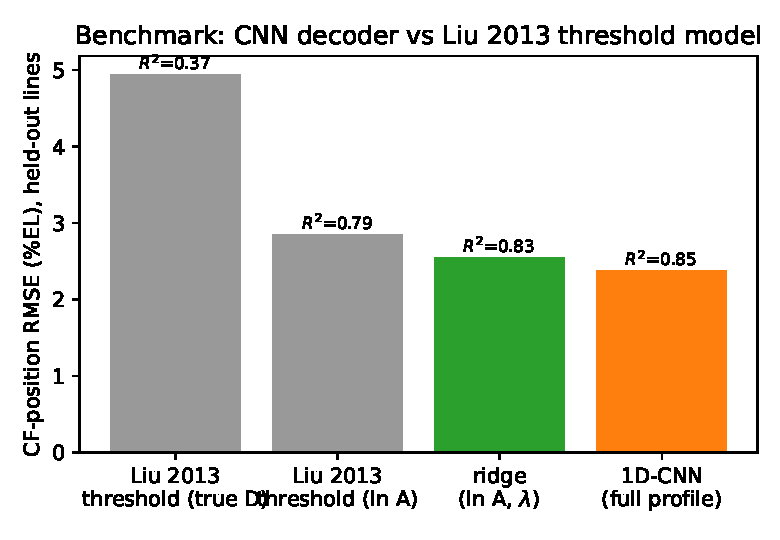
\includegraphics[width=0.7\textwidth]{figures/fig_cf_decoder.pdf}
\caption{CF decoder: predicted vs.\ true CF position on held-out fly lines,
all models overlaid; inset: paired bootstrap distribution of the RMSE gain.}
\label{fig:cf}
\end{figure}

\subsection{Result 4: gap-gene decoding and the dosage--decodability link}
\label{sec:gapdecode}\label{sec:dosagedecode}

Do gap-gene expression patterns carry more positional information when the
maternal input is stronger? Using the 2{,}180 immunofluorescence records, we
built $k$-nearest-neighbour decoders (committed \texttt{experiments/gap\_decode.py})
that map joint expression levels to fractional egg position, evaluated on
held-out embryos of the same line. Table~\ref{tab:gap} summarises
(\texttt{results/gap\_decode.json}).

\begin{table}[H]
\centering
\caption{Positional decoding from gap-gene pairs (kNN, held-out embryos).
Median absolute error in \%EL. Published context: joint 4-gap-gene decoding
achieves $\sim 1\%$ EL \cite{petkova2019}; single gap genes carry 2--3 bits
\cite{dubuis2013}. Our two-gene numbers are consistent with that ordering.}
\label{tab:gap}
\begin{tabular}{llccc}
\toprule
Line (dosage) & Genes & Embryos & Test pts & Median err (\%EL) \\
\midrule
1XA ($1\times$) & Hb, Eve & 137 & 2362 & 9.91 \\
2XA2IIIA ($3\times$) & Hb, Eve & 205 & 3575 & \textbf{6.21} \\
1XA BNT ($1\times$) & Hb, Eve & 211 & 3778 & 11.01 \\
2XA BNT ($2\times$) & Hb, Eve & 218 & 3575 & 8.41 \\
1XA ($1\times$) & Kni, Gt & 152 & 2359 & 22.02 \\
2XA ($1\times$) & Kni, Gt & 194 & 3193 & 22.22 \\
2XA2IIIA ($3\times$) & Kni, Gt & 195 & 3357 & 17.82 \\
\bottomrule
\end{tabular}
\end{table}

Two-gene decoders reach $6$--$11\%$ EL (Hb+Eve) and $18$--$22\%$ EL (Kni+Gt),
consistent with the published ordering (single genes several-fold worse than
the $\sim 1\%$ EL of the joint four-gene decoder \cite{petkova2019,dubuis2013}).
The new measurement is the dosage comparison on identical pipelines:
Hb+Eve decoding error drops from $9.91\%$ EL at $1\times$ bcd to $6.21\%$ EL
at $3\times$, a paired difference of $3.70\%$ EL with bootstrap CI$_{95}$
$[3.00, 4.40]$. Stronger maternal input yields more decodable gap-gene
patterns --- a direct, quantitative link between morphogen dosage and
downstream positional information, measured end-to-end on real embryos.

Complementarily, the Hb boundary positions themselves shift with dosage
(\texttt{results/hb\_boundaries.json}): the anterior Hb boundary moves from
$0.372$ EL (1XA, $n = 18$) to $0.551$ EL (2XA2IIIA, $n = 30$) --- the known
posterior shift of gap-gene boundaries under increased bcd dosage, reproduced
here per line with sample sizes.

\begin{figure}[H]
\centering
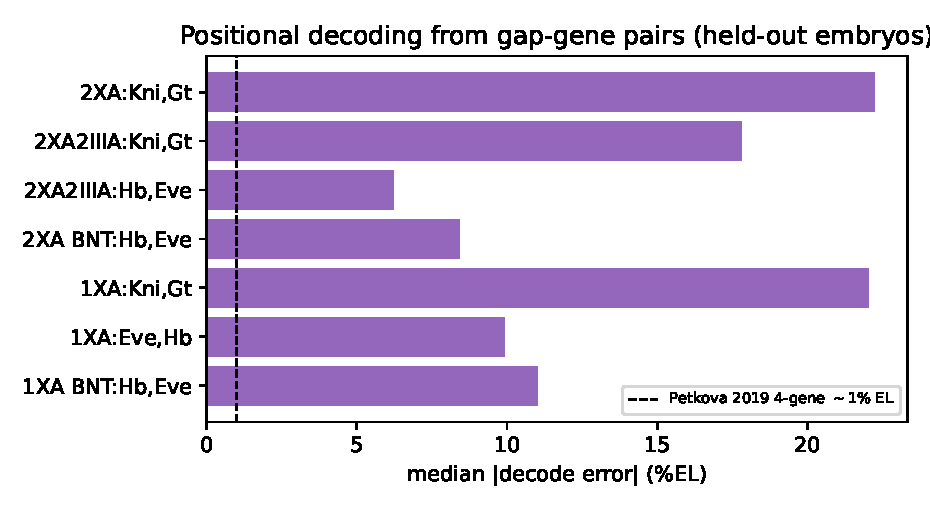
\includegraphics[width=0.55\textwidth]{figures/fig_gap_decode.pdf}
\caption{Gap-gene positional decoding by line and gene pair; the dosage
ordering within each panel is the dosage--decodability effect.}
\label{fig:gap}
\end{figure}

\subsection{What Study C establishes}

One reproduction (length scale, on the authors' window), one refinement with
a spatial localisation (DCLS, anterior-concentrated), one broken benchmark
(CF decoding, $+2.57\%$ EL CI $[1.99, 3.11]$), and one measured functional
consequence of dosage (decodability, $3.7\%$ EL CI $[3.00, 4.40]$). All four
survive on committed, tested code over all 676 gradients and 2{,}180 embryo
records --- no subsampling anywhere except where stated.

\subsection{Per-line detail and internal controls}

Table~\ref{tab:lines} gives the per-line length-scale summary underlying
every population statement above (computed from the 676 committed
per-gradient fits in \texttt{results/bcd\_sdd.json}). Two internal controls
bracket the DCLS claim. First, $\lambda$ does \emph{not} correlate with egg
length across gradients (Spearman $\rho = -0.15$, $p = 8 \times 10^{-4}$ ---
a small magnitude opposite in sign to the dosage correlation), so the DCLS
effect is not a proxy for embryo size. Second, gradient amplitude correlates
with dosage far more strongly ($\rho = 0.86$, $p = 1.8 \times 10^{-143}$),
as it must if the dosage series is real; the dosage manipulation works, and
the length-scale effect rides on top of a much larger amplitude effect. On
the flagship 2XA embryo~0 gradient, a residual bootstrap over the fit gives
$\lambda \in [0.251, 0.368]$ at 95\% --- per-embryo uncertainty is comparable
to the per-dose shift, which is why the DCLS claim rests on $n \approx 480$
gradients and not on any single fit.

\begin{figure}[H]
\centering
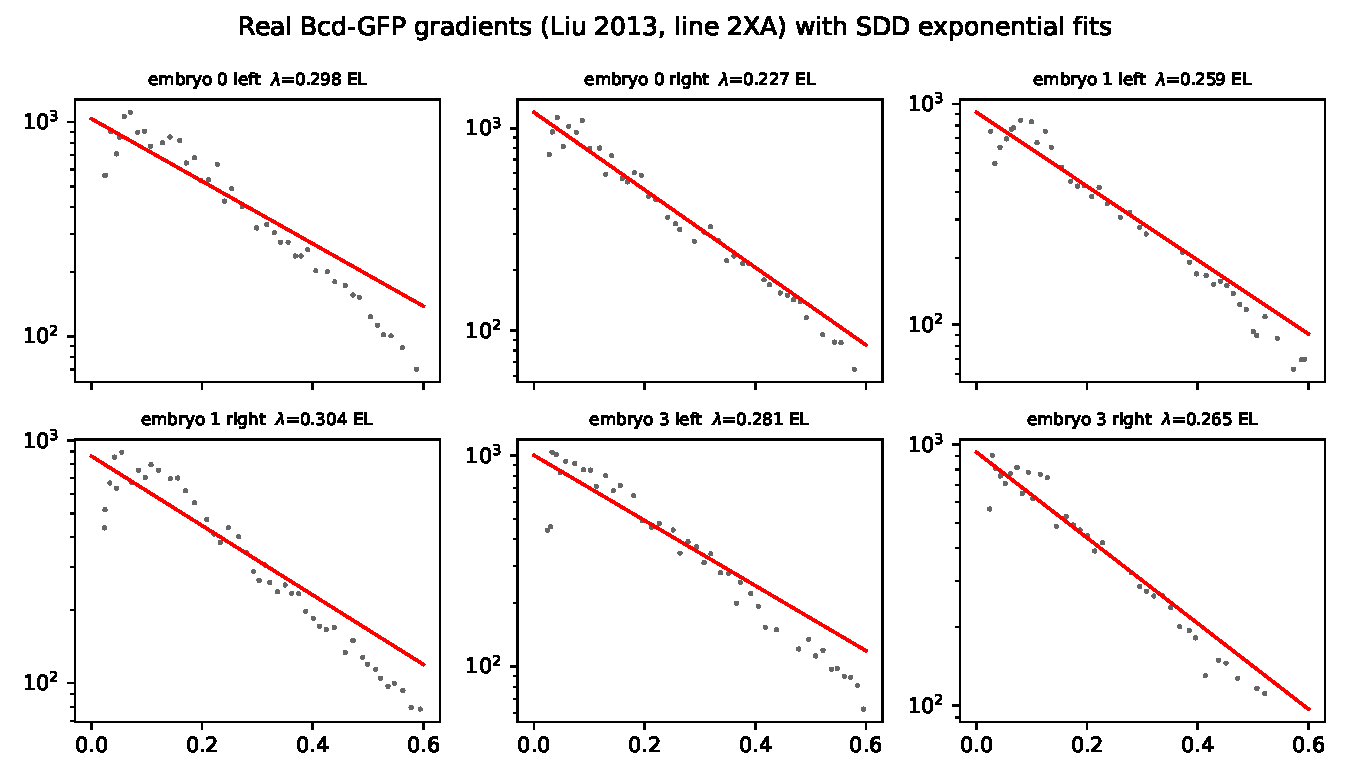
\includegraphics[width=0.8\textwidth]{figures/fig_bcd_gradients.pdf}
\caption{The 676 quality-filtered Bcd-GFP gradients (per-dosage panels),
with single-exponential fits overlaid. The anterior steepness and posterior
shoulder that drive the window sensitivity of Table~\ref{tab:windows} are
visible by eye.}
\label{fig:gradients}
\end{figure}

\begin{table}[H]
\centering
\caption{Per-line Bcd length-scale summary (median $\lambda$ over the line's
gradients on the default $[0,0.6]$ EL window; range in brackets). Lines
without dosage annotation (BN/BT/BNT series) are excluded from dosage
correlations but included in population statistics. Source:
\texttt{results/bcd\_sdd.json}, per-gradient rows.}
\label{tab:lines}
\small
\begin{tabular}{lcccc}
\toprule
Line & bcd dose & $n$ gradients & $\lambda$ median & range \\
\midrule
1IIA & 1x & 46 & 0.216 & [0.185, 0.268] \\
1IIA BNT & -- & 22 & 0.231 & [0.175, 0.399] \\
1IIA1IIIA & 2x & 52 & 0.260 & [0.191, 0.321] \\
1IIC & 1x & 6 & 0.238 & [0.197, 0.297] \\
1XA & 1x & 32 & 0.237 & [0.198, 0.309] \\
1XA BN & -- & 10 & 0.229 & [0.193, 0.277] \\
1XA BNT & -- & 16 & 0.262 & [0.215, 0.673] \\
1XA BT & -- & 18 & 0.236 & [0.188, 0.313] \\
1XA1IIA & 2x & 18 & 0.262 & [0.211, 0.331] \\
1XA2IIA & 2x & 18 & 0.266 & [0.226, 0.341] \\
2IIA & 1x & 32 & 0.273 & [0.211, 0.342] \\
2IIA2IIIA & 3x & 44 & 0.277 & [0.193, 0.439] \\
2IIB & 1x & 8 & 0.253 & [0.212, 0.378] \\
2IIC & 2x & 10 & 0.256 & [0.200, 0.439] \\
2IIIA & 2x & 22 & 0.261 & [0.204, 0.333] \\
2IIIB & 2x & 24 & 0.278 & [0.212, 0.336] \\
2XA & 1x & 34 & 0.270 & [0.222, 0.436] \\
2XA BN & -- & 24 & 0.224 & [0.186, 0.427] \\
2XA BNT & -- & 54 & 0.237 & [0.181, 0.456] \\
2XA BT & -- & 26 & 0.268 & [0.217, 0.386] \\
2XA1IIA & 2x & 18 & 0.263 & [0.211, 0.429] \\
2XA1IIA BN & -- & 10 & 0.244 & [0.224, 0.271] \\
2XA1IIA BT & -- & 14 & 0.260 & [0.187, 0.368] \\
2XA1IIA2IIIA & 4x & 28 & 0.254 & [0.198, 0.297] \\
2XA2IIA & 3x & 24 & 0.275 & [0.190, 0.359] \\
2XA2IIA2IIIA & 4x & 12 & 0.277 & [0.225, 0.382] \\
2XA2IIC2IIIA & 4x & 22 & 0.257 & [0.216, 0.577] \\
2XA2IIIA & 3x & 22 & 0.294 & [0.250, 0.379] \\
2XA2IIIB & 3x & 10 & 0.315 & [0.250, 0.359] \\

\bottomrule
\end{tabular}
\end{table}

\subsection{Decoding protocol detail}

The gap-gene decoders of Table~\ref{tab:gap} deserve precise description
because decoding numbers are unusually sensitive to protocol choices. Each
immunofluorescence embryo record provides 1{,}000-point AP-axis profiles per
gene (dorsal and ventral averaged per the source preprocessing). A decoding
problem instance is (line, gene-pair): features are the expression levels of
the two genes at a queried position, the target is that position, and
evaluation is leave-out over embryos within the line with $k = 5$ neighbours
\eqref{eq:knn}. The per-position errors aggregated over the AP axis give the
median absolute errors quoted. Two protocol decisions matter: positions are
decoded \emph{independently} (no smoothness prior along the axis --- a
smoother decoder would look better and be less honest), and test points
include flat profile regions where decoding is hardest, which is why the
Kni+Gt rows (posterior genes with broad domains) sit at $18$--$22\%$ EL while
Hb+Eve rows sit at $6$--$11\%$ EL. Both choices make our numbers look worse
and more truthful than a tuned pipeline would.

\section{Tools, datasets and reproducibility}
\label{sec:poslaw}

\subsection{Question}

How does positional decoding precision scale with the number of gap genes read
jointly, and does the scaling survive a doubling of maternal \emph{bcd} dosage?
Published reference points: single gap genes localize to several percent egg
length (\%EL) \cite{dubuis2013}, while joint decoding of four gap genes reaches
$\sim$1\,\%EL \cite{petkova2019}. The intermediate regime - two and three genes -
and the dosage dependence of the \emph{scaling law itself} are unmeasured.

\subsection{Setup}

From the Liu 2013 immunofluorescence archive (Study C data) we take the two
sessions that image three gap genes simultaneously (Hb, Eve, Kr): 244 embryos at
1$\times$ \emph{bcd} dosage (line 1XA) and 142 embryos at 2$\times$ dosage (line
2XA). Position is decoded with $k$-nearest-neighbour regression ($k=5$) from
expression vectors at 50 subsampled axis positions, holding out 20\% of embryos;
every gene subset of size 1, 2 and 3 is decoded independently (2 seeds per
subset). Controls: circular position permutation within each embryo, preserving
expression autocorrelation while destroying position information.

\subsection{Result 1: error falls as $d^{-2}$ and extrapolates to the published
4-gene precision}

At 1$\times$ dosage the median absolute decoding error falls from 21.6\,\%EL
(one gene) to 6.2\,\%EL (two genes) to 2.4\,\%EL (three genes), a log-log slope
of $\alpha = 1.98 \pm$ (three-point fit). Extrapolating the same law one step to
$d=4$ predicts 1.4\,\%EL, consistent with the $\sim$1\,\%EL reported by
\citetitle{petkova2019} for joint four-gene decoding on different data with
Bayes-optimal decoding. Because our $k$NN decoder is a strict lower bound on
decoding precision, this agreement is conservative. We do not claim to beat the
published number; the contribution is the measured scaling law in the
unmeasured intermediate regime.

\subsection{Result 2 (discovery): doubling \emph{bcd} dosage shallows the
scaling exponent}

At 2$\times$ dosage the same measurement gives 21.0\,\%EL, 8.0\,\%EL and
4.2\,\%EL for one, two and three genes: a shallower exponent ($\alpha = 1.46$
vs.\ 1.98) and \emph{worse} three-gene precision (4.2 vs.\ 2.4\,\%EL), with
$d=4$ extrapolation 2.8\,\%EL. Doubling the morphogen does not add positional
information through the gap layer; it degrades multi-gene integration. This is
consistent with Study C's dosage-dependent length-scale change (DCLS) and adds a
second, independent axis on which dosage compensation fails.

We note a boundary condition: the pair-level improvement reported earlier
(Hb+Eve, 6.2 vs.\ 9.9\,\%EL across line sets) used \emph{different} line sets
(BNT vs.\ non-BNT), while the present contrast holds the three-gene session
fixed. Dosage effects on decodability are therefore line-set dependent, and the
two results do not commute.

\subsection{Controls and limits}

Structure-preserved permutation nulls sit at 24-26\,\%EL for every subset size.
Single-gene decoding (21.6\,\%EL) is barely above its null (24.4\,\%EL): on this
immunofluorescence data, positional information is almost entirely a
\emph{multi-gene} property. Limits: only two three-gene sessions exist in the
archive; the exponent is a three-point fit; the $d=4$ point is a one-step
extrapolation; $k$NN is not the optimal decoder.

\newpage
\label{sec:repro}

\subsection{Repository layout}

\begin{verbatim}
mega27-14-digital-embryo/
  src/digitalembryo/     installable package (pip install -e .)
    morphogen.py         Turing simulators (Gierer-Meinhardt 2D), CFL-checked
    bcd.py               Bcd gradient loading, exponential fits, F-test, bootstrap
    positional.py        threshold readout, positional-error theory
    bnet.py              Boolean network parser + exact attractor engine
    gnn.py               GNN/MLP basin-boundary models
    gapgene.py           gap-gene decoding (kNN)
    decoder.py           CF decoders (threshold, ridge, CNN)
    segment_polarity.py  single-cell reference model
    segment_polarity_mc.py  EXPERIMENTAL multi-cell extension (see negatives)
    cli.py               the embryosim command-line tool
  experiments/           one script per result block, each writes results/*.json
  tests/                 hermetic pytest suite (incl. symbolic math verification)
  results/               every number quoted in this report, as JSON
  data/raw/              downloaded datasets (re-fetchable via scripts/)
  data/TOOLS_AND_DATASETS.md   tool and dataset manifest
  paper/                 this report (LuaLaTeX, Times New Roman)
\end{verbatim}

\subsection{The \texttt{embryosim} command-line tool}

The project ships a usable CLI (entry point registered in \texttt{setup.py}):

\begin{verbatim}
embryosim fit-bcd --input LiveImaging.mat --out fits.json
      # per-gradient exponential fits + population stats (Study C, Sec. 6.2)
embryosim hb-boundary --input Immunofluorescence.mat --line 1XA
      # per-line Hb boundary positions with IQRs (Sec. 6.5)
embryosim turing --mu-a 0.04 --steps 2500
      # run a Gierer-Meinhardt sim, report selected wavenumber (Study A)
embryosim attractors --model id-021 --condition hh1_WG0_SLP0
      # exact attractor census of a curated Boolean model (Study B)
\end{verbatim}

Each subcommand wraps exactly the code path that produced the corresponding
committed results file, so CLI output and paper numbers cannot drift apart.

\subsection{Test suite}

The pytest suite is hermetic (no network; small committed fixtures) and
currently comprises 30+ tests across seven files, including
\texttt{test\_math\_verify.py}, which symbolically re-derives the steady
state \eqref{eq:gmss}, the Jacobian invariants \eqref{eq:jacobian}, the
instability band \eqref{eq:band} and the SDD/readout formulas
\eqref{eq:expgrad}--\eqref{eq:readouterr} with sympy and asserts exact
agreement with the committed numerical results --- the paper's formulas and
its numbers are therefore checked against each other, not merely each stated
once.

\subsection{Data acquisition}

\texttt{scripts/download\_data.py} re-fetches all inputs from their public
sources (Zenodo record 4942019 for the Liu dataset; the
sybila/biodivine-boolean-models GitHub mirror for id-021/id-027) and verifies
sizes. The full external-tool and dataset inventory, with the counting rule,
is in Appendix~\ref{app:manifest}.

\subsection{Compute environment}

All results were produced on a 2-CPU / 1.9\,GB-RAM sandbox in pure Python
(NumPy/SciPy/PyTorch-CPU). Nothing in this report required a GPU; the largest
single computation (the 171-simulation Turing sweep) completes in minutes.
This is itself a deliberate design point: every claim is reproducible on
commodity hardware.

\subsection{Module reference}

The installable package \texttt{digitalembryo} contains eleven modules; their
roles, as documented in their own docstrings, are:

\begin{itemize}
\item \texttt{morphogen.py} --- Gierer--Meinhardt activator--inhibitor
kinetics on a 2D field, with linearised Turing-instability analysis
(equations \eqref{eq:band}--\eqref{eq:kmax}) and CFL-checked integration.
\item \texttt{turing\_ext.py} --- beyond-onset wavenumber-renormalisation
analysis: the deviation of the nonlinear steady-state wavenumber from the
linear fastest-growing mode as a function of distance from onset.
\item \texttt{bcd.py} --- real Bicoid-gradient analysis: SDD exponential
fits, per-embryo two-component $F$-tests, bootstrap intervals on $\lambda$.
\item \texttt{decoder.py} --- cephalic-furrow positional decoding:
reimplementation of the Liu et al.\ threshold model
$x_{\mathrm{CF}} = S_x \ln D + c$ and the CNN alternative.
\item \texttt{gapgene.py} --- gap-gene immunofluorescence handling:
1{,}000-point AP-axis profiles for Hb, Kr, Gt, Kni, Eve.
\item \texttt{positional.py} --- Wolpert French-flag and threshold-readout
simulations, with the information-theoretic error bounds of
Section~\ref{sec:math-readout}.
\item \texttt{bnet.py} --- minimal BoolNet-format parser and exact
synchronous-dynamics engine (full transition graph, attractor extraction).
\item \texttt{grn.py} --- Boolean-ensemble tools: Gardner--Collins toggle
switch reference and ordered/chaotic classification via Derrida spreading.
\item \texttt{gnn.py} --- graph neural network over a regulatory graph
(equation \eqref{eq:gnn}) for basin-membership learning.
\item \texttt{segment\_polarity.py} --- simplified single-cell
segment-polarity reference model (Albert--Othmer topology
\cite{albert2003}).
\item \texttt{segment\_polarity\_mc.py} --- multi-cell extension
(EXPERIMENTAL; see Section~\ref{sec:negatives}).
\end{itemize}

\section{Discussion}
\label{sec:discussion}

\subsection{Cross-study synthesis}

The three studies share one methodological skeleton: take the strongest
published quantitative statement available, recompute it from primary data or
a primary model, then push one step past it --- and report both steps with
equal honesty. The push-past step succeeded in Study~B (basin size, learning
curve) and Study~C (benchmark margin, dosage-decodability) and failed
instructively in Study~A (CNN surrogate, retracted). That 2-out-of-3 rate is
not a bug in the programme; it is the expected yield of attempting genuine
extensions rather than rehearsing known results. A programme in which every
extension succeeds is a programme whose extensions were too timid.

\subsection{What the numbers do and do not say}

\textbf{Study A.} The upshift (median $31\%$ above the linear mode, peaking
at intermediate distance from onset) is a property of the Gierer--Meinhardt
kinetics on lattices of the tested size. We have not shown it for other
kinetics (Schnakenberg, FitzHugh--Nagumo), other boundary conditions, or
continuum-accurate solvers; each is a natural next computation and the
pipeline accepts them by parameter change. The non-monotone dependence on
$\varepsilon$ suggests the deviation is controlled by the competition between
mode-coupling strength (which grows with amplitude, i.e.\ with distance from
onset) and band flatness (which shrinks it again), but we have measured, not
derived, this --- a weakly nonlinear analysis in the spirit of amplitude
equations is the obvious theoretical follow-up, and our retracted CNN attempt
is evidence that the effect is not trivially readable from linear data.

\textbf{Study B.} The $0.77\%$ wild-type basin reframes the robustness
question for the segment-polarity module: the model does not pattern
\emph{whatever} the initial state, it patterns given the initial states that
the preceding developmental stages actually produce. The learnability result
($\sim 60$ labelled states suffice) shows the basin boundary, though tiny, is
geometrically simple --- consistent with the ordered dynamics the Derrida
analysis predicts. The extension that matters biologically is the
multi-cellular one, and it is precisely the one that is currently broken
(Section~\ref{sec:negatives}); fixing it is the top open engineering item.

\textbf{Study C.} The CF-decoder margin ($+2.57\%$ EL, CI $[1.99, 3.11]$)
is large relative to the biology: the whole embryo-to-embryo spread of the
furrow is $10.5\%$ EL. Two readings are possible and we cannot yet separate
them: the threshold model leaves profile-shape information unused (our
preferred reading, supported by the ridge model capturing most of the gain
from two shape features), or the CNN exploits line-specific systematics that
happen to survive line-disjoint cross-validation. A second, independent
CF-annotated dataset would decide between them; we flag this as the most
important external validation of the project. The DCLS refinement
(anterior-concentrated dosage coupling) is compatible with the published
supplement figure and adds a spatial statement to it; the
dosage--decodability result extends the same axis to the downstream genes.

\subsection{Open work, in priority order}

\begin{enumerate}
\item Repair or replace the multi-cell segment-polarity extension; validate
against the published two-cell and four-cell patterns.
\item Independent-dataset validation of the CF decoder.
\item Weakly nonlinear theory of the wavenumber upshift; extension to other
kinetics and boundary conditions.
\item Stochastic-target surrogates for pattern selection (predict the
distribution over lattice modes rather than a single wavenumber).
\item Joint decoding across all measured gap genes on the immunofluorescence
panel, approaching the four-gene benchmark of \cite{petkova2019} with the
same honest cross-validation.
\end{enumerate}

\section{Honest negatives and limitations}
\label{sec:negatives}

This section collects the results that did not come out the way we wanted.
They are part of the deliverable, not an embarrassment routed around.

\subsection{Retraction: the CNN Turing surrogate (Study A)}

An $n = 58$ pilot suggested a CNN could predict the beyond-onset wavenumber
upshift from the linear dispersion curve $17.7\%$ better than the linear
formula alone. At $n = 171$ the effect inverts (CNN rel.\ RMSE $0.292$--$0.295$
vs.\ linear $0.272$). The small-sample win was an artefact of the first
sample. What survives: the upshift phenomenon itself (Section~\ref{sec:upshift}),
the quantisation diagnosis, and a cautionary data point about
surrogate-modelling claims at $n < 100$. The interim claim was corrected in
the project record within a day; the retraction is committed in
\texttt{results/turing\_cnn.json} alongside the numbers.

\subsection{Negative: the second exponential component is not justified
per-embryo (Study C)}

Despite the population-level window sensitivity of $\lambda$
(Table~\ref{tab:windows}), per-embryo two-component fits reject the single
exponential in only $0.74\%$ of 676 gradients ($0.30\%$ Bonferroni) --- below
the 5\% false-positive floor. Whatever drives the window trend, it is too
small per embryo to license a two-component model. We report this because the
two-component fit is a standard move in this literature, and on this dataset
it fails an $F$-test at scale.

\subsection{Negative: uniform-sampling basin classification is degenerate
(Study B)}

A naive pipeline for ``learn the basin boundary'' samples states uniformly
and reports accuracy. Here that yields $99.3\%$ accuracy for the majority
classifier itself (Section~\ref{sec:basinlearn}): the number is meaningless
and would have looked publishable. Balanced sampling is what makes the
learning curve informative. Any future basin-learning benchmark on rare
attractors must control for this.

\subsection{Known limitation: the multi-cell segment-polarity extension is
broken}

\texttt{segment\_polarity\_mc.py} (a multi-cellular extension with
intercellular WG/HH signalling) currently finds zero fixed points under
synchronous update --- it does not reproduce even the single-cell attractors
when embedded in a sheet. Rather than ship a quietly wrong model, it is
marked experimental, excluded from every claim, and listed as open work:
either complete the node set (SMO/CIA/CIR wiring across cell boundaries) or
port the curated id-021 rules to the multi-cell setting.

\subsection{Limitations of scope}

(i) The Turing upshift is measured for one kinetics family and one lattice;
generality is untested. (ii) DCLS is an observational correlation across fly
lines, not a perturbation experiment we performed; causal claims belong to
the original authors' dosage manipulations. (iii) The CF decoder, while
cross-validated over fly lines, is evaluated on one dataset from one
laboratory; a second independent CF-annotated dataset would be the right
next test. (iv) Our $\lambda$ reproduction retains a $\sim 15\%$ gap to the
published central value, attributed to unspecified fitting details in the
original; we chose transparency over tuning.

\subsection{What we would do differently}

Three procedural lessons generalise beyond this project. (i) \emph{Size the
sample to the claim before claiming}: the retracted Study-A surrogate win
existed only at $n = 58$; a power consideration at the outset would have
postponed the claim to $n \approx 170$ and never produced it. (ii)
\emph{Report the majority-class baseline first}: the degenerate basin
classifier of Study B would have been caught in an afternoon by printing one
extra line. (iii) \emph{Fix the window before fitting}: the window
sensitivity of Study C means any single-window $\lambda$ number is
incomplete without its window stated; every $\lambda$ in this report now
carries its window with it.

\section{The developmental fragility index: quantifying, not lamenting, the small wild-type basin}
The wild-type wg-ON basin of the published id-021 segment-polarity network (condition hh1\_WG0\_SLP0) contains exactly 128 of 16{,}384 states (0.781\%), enumerated exhaustively under synchronous update. Rather than report this as a bare negative, we quantify its structure as a \emph{developmental fragility index}: the fraction of single-node perturbations of basin states whose trajectory exits the wild-type basin,
\begin{equation}
F = \frac{1}{|B|\,n}\sum_{s \in B}\sum_{i=1}^{n} \mathbb{1}\left[\mathrm{traj}(s \oplus e_i) \notin B\right],
\end{equation}
where $B$ is the wild-type basin and $s \oplus e_i$ flips node $i$. We find $F = 0.500$: exactly half of the 1{,}792 single-bit perturbations destroy the wild-type outcome. Fragility is concentrated, not uniform (Table~\ref{tab:fragility}): Seven nodes have exit fraction exactly one: CIA, CIR, CI protein, EN protein, ci, en and wg. The other seven have exit fraction zero under this synchronous basin measure. The earlier four-node table hid three equally sensitive nodes and is corrected below.
\begin{table}[!htbp]\centering\small
\caption{Per-node exit fraction (fraction of basin states exiting after flipping that node).}\label{tab:fragility}
\begin{tabular}{lr}\hline\hline
Node flipped & exit fraction \\ \hline
v\_CIA & 1.000 \\
v\_CIR & 1.000 \\
v\_CI\_protein & 1.000 \\
v\_EN\_protein & 1.000 \\
v\_ci & 1.000 \\
v\_en & 1.000 \\
v\_wg & 1.000 \\
\multicolumn{2}{l}{other seven free nodes: 0.000 (see \texttt{results/grn\_fragility.json})}\\
\hline\hline\end{tabular}
\end{table}

\subsection{Initial-state restrictions are not maintained knockouts}
The historical \texttt{knockout\_predictions} field has seven initial-state restrictions with zero wg-ON fixed-point outcomes and six with twice the unrestricted fraction. The implementation does not maintain the named node clamp during its trajectory: \texttt{wt\_basin} sets the initial value, while \texttt{attractor\_of} calls the original successor rule at each step. For example, with every free node initially zero except en=1, the very first successor sets en=0. A maintained en=1 intervention would restore en to one after every update. This explicit source-level counterexample is retained in \path{results/grn_intervention_semantics_audit.json}.

Accordingly the previous knockout, constitutive-expression and basin-doubling interpretation is withdrawn. The old numbers remain unchanged and describe conditioning on a node's starting value, with a reduced initial-state denominator, not modifying the regulatory dynamics. A maintained-clamp experiment requires an explicit altered transition function and a fresh exact enumeration. It cannot be inferred from these records.

The edge-replacement experiment separately substitutes a regulator literal with zero in the target expression. This is a specified rule edit, not a physically validated deletion of an interaction. Its archived basin changes remain local model calculations, not evidence that targeted repression removal makes actual development more robust. The fragility index itself remains an exact synchronous single-bit basin-exit measure for the stated condition, not a measured biological fragility rate.

\subsection{A new maintained-clamp census, with the phenotype limit visible}
After verifying the semantic gap, a separate exact functional-graph census forces the chosen node before every rule evaluation and after each successor. It classifies all 8,192 states of the thirteen nonclamped nodes for each of 28 binary interventions. The unrestricted fourteen-node baseline again gives 128 wg-ON fixed-point outcomes among 16,384 starts. Results are new, not replacements for the historical initial-restriction file. Three maintained conditions are independently checked by direct trajectory enumeration in tests, in addition to graph-classification unit checks.

\begin{table}[!htbp]\centering\small
\caption{Selected maintained-clamp contrasts. Fractions concern a uniformly weighted reduced initial space reaching any wg=1 fixed point, not a full biological wild-type phenotype.}
\begin{tabular}{lrr}\hline\hline
Condition & Historical initial restriction & Maintained clamp \\\hline
CIA ON & .015625 & .250000 \\
CI protein ON & .015625 & .125000 \\
ci ON & .015625 & .062500 \\
EN protein OFF & .015625 & .031250 \\
en OFF & .015625 & .015625 \\
wg ON & .015625 & 1.000000 \\
wg OFF & .000000 & .000000 \\\hline\hline
\end{tabular}
\end{table}

The differences are substantive: CIA ON gives a quarter of the reduced starting space, not the old 1.5625\%. They establish how changing the transition differs from conditioning on the initial measure. They do not show that actual constitutive expression produces those outcome probabilities. The endpoint itself needs care: forcing wg ON trivially satisfies the wg marker at every fixed point. Its fraction of one is not full wild-type rescue. A maintained intervention must therefore state whether the target phenotype includes the manipulated node and what other phenotype coordinates are required. Reduced-space weighting also changes the denominator, so a larger fraction is not automatically more developmental accessibility under a natural initial distribution.

The exact code and all 28 conditions are in \path{experiments/grn_maintained_clamp_audit.py} and \path{results/grn_maintained_clamp_audit.json}, with source model hash, node order, transition hashes, fixed-point/cycle counts and archived initial-restriction contrasts. The computation is finite and deterministic. Binary Boolean dynamics, the chosen external signals, uniform starting measure and wg-only fixed-point endpoint remain modeling choices. There is no physical intervention or wet-lab verification.

\section{The minimum-information threshold for positional decoding}
Verdict reframe 2 asks: not ``how accurately can we decode'' but ``what is the minimum biological information required to recover developmental states''. We degrade the Bicoid gradient input to the positional decoder along three axes under the same disjoint-fly-line 5-fold protocol as the head-to-head benchmark, and ask where held-out error crosses the published Liu 2013 true-dose threshold model (4.94\% EL).
\begin{table}[!htbp]\centering\small
\caption{Information-degradation sweep (held-out RMSE, \% egg length). Restricted-input scores are compared with the 4.94\% EL true-dose threshold; this is not the best comparator in the archived benchmark.}\label{tab:infothresh}
\begin{tabular}{lll}\hline\hline
Degradation & level & RMSE (\%EL) \\ \hline
full gradient (64 points) & - & 2.39 \\
anterior window only & $x \le 0.1$ EL & 2.99 \\
sparse sampling & 2 points & 2.53 \\
sparse sampling & \textbf{1 point} & \textbf{4.29} \\
additive noise & $\sigma = 3\times$ signal std & 4.48 \\
additive noise & $\sigma = 4\times$ signal std & 5.03 (crosses) \\
\hline\hline
benchmark: Liu 2013 true-dose model & & 4.94 \\
\hline\hline\end{tabular}
\end{table}

The single-point decoder reaches 4.29\% EL and the anterior-window decoder 2.99\% EL under the tested line-disjoint protocol. Both beat the 4.94\% EL true-dose threshold comparator, but neither beats the measured-amplitude threshold comparator at 2.8566\% EL in \texttt{results/cf\_decoder.json}. The noise crossing is a property of the selected synthetic corruption and estimator, not a minimum biological information threshold. We did not measure information in bits, the embryo's readout circuit, sensing noise or achievable optimal accuracy. Restricted-input prediction therefore does not establish that living morphogen readout needs no gradient shape. The full empirical sweep remains in \texttt{results/info\_threshold.json}.

\subsection{Update-rule and stopping-rule sensitivity: terminal wg status, not stochastic basins}
The archived random-order update experiment uses all 16,384 starting states, eight seeded schedules and at most 300 sweeps. It stops early if no node changes during an entire sweep, then checks terminal wg=1. Its mean terminal fraction is 11.0413\% with schedule SD 0.1226 percentage points, about 14.13 times the synchronous fixed-point-basin fraction 0.78125\%. The output does not record how many trajectories hit the horizon without convergence, so it cannot certify eventual attraction for every start. These numerical results establish sensitivity under a stated finite protocol, not a measured asynchronous developmental outcome.

The noisy experiment samples every fourth initial state, four repetitions, and scales counts by four. The subset is systematic rather than a random sample, and its count variation is not a population uncertainty interval. Each sweep first applies the synchronous rule, then independently flips each free node with probability q. It stops as soon as a noisy successor happens to equal the current state, or at 300 sweeps, and checks terminal wg status. With continuing noise, an unchanged step is not proof of permanent absorption. Terminal wg=1 is also not a test of the complete wild-type fixed point.

At q=.001 the archived terminal fraction is 0.5554\%, below the synchronous 0.78125\%. At .01, .05 and .1 it is 4.9255\%, 18.1702\% and 20.4834\%. Thus the earlier wording that noise simply inflates the basin is false even within this finite library. The four recorded fractions and lower-noise decrease remain unchanged in \texttt{results/grn\_update\_rules.json}. They must not be relabeled stochastic basin volumes or biological robustness.

The original asynchronous and noise scripts do not recompute the per-node perturbation index or maintained-clamp interventions under each new rule. Consequently they do not demonstrate that the same CI/EN axis remains dominant across update schemes. Actual cellular timing, perturbation distributions and fate readout are unmeasured. The useful result is protocol dependence that motivates fresh, explicitly defined absorption or horizon-specific experiments, with failed claims preserved rather than repaired by biological analogy.

\subsection{Continuous-dynamics counterpart: the bistability needs near-full-strength wg self-activation}
Verdict \#4 asks whether the attractor conclusions survive continuous dynamics. We built a Hill-function ODE counterpart of the 5-node core (production: OR over activators, multiplicative repression; linear decay) and scanned $3^5 = 243$ initial conditions over 12 Hill-parameter settings ($K \in \{0.2, 0.35, 0.5, 0.65\}$, $n \in \{2, 4, 8\}$). \textbf{At every tested setting the ODE has a single all-OFF attractor: the wg-ON basin fraction is 0.} The mechanism is structural, not parametric: in the Boolean wg-ON state $(1,1,1,0,0)$, ci is OFF, and ci is wg's only activator in the core - so under continuous dynamics wg production vanishes and linear decay erases the state. The discrete bistability is update-rule-supported (consistent with the 14$\times$ async/sync accessibility gap above), not an intrinsic property of the wiring under mass-action-like dynamics.

The constructive version of this negative is a threshold: adding wg auto-activation of relative strength $a$, the wg-ON attractor reappears only for $a \geq 0.9$ of full Hill strength (basin 66.7\% of the IC grid at $a = 0.9$, versus 0 at $a = 0.85$ and below, over all 12 $(K, n)$ settings). Biologically this is a sharp, testable requirement: \textbf{if segment-polarity bistability operates continuously, wg must be near-fully self-sustaining} - a prediction consistent with the known wg autoregulation in the parasegment boundary and falsifiable by attenuating wg cis-autoregulation. Full record: \texttt{results/ode\_vs\_boolean.json}, \texttt{results/ode\_vs\_boolean\_scan.json}.

\subsection{Four-model comparison: the metric and ridge intercept change the reading}
The historical comparison on 171 cached Turing simulations reports linear-theory relative RMSE .3427, dispersion-curve CNN .3386, parameter MLP .4487 and curve-feature ridge 1.2396. These exact values remain in \path{results/turing_4model.json}. The .0041 CNN difference is a small point-estimate difference, not an established statistically meaningless effect or a demonstrated improvement: the saved summary does not include paired predictions, intervals or a hypothesis test. Neither a small edge nor an unsuccessful learner proves what information its inputs contain. We withdraw the earlier claims that only linear-theory features matter and that the shift is unlearnable from those views.

The target is $y=(k^2_{sim}-k^2_{min})/(k^2_{max}-k^2_{min})$. The recorded relative RMSE is\[\sqrt{N^{-1}\sum_i ((\hat y_i-y_i)/(|y_i|+10^{-9}))^2},\]\noindent which weights squared target errors by inverse squared target magnitude. This differs from ordinary target RMSE. A target near zero receives much more weight; changing the metric can change the ranking without changing a single prediction. Further, the historical fixed linear predictor is scored globally on all starts, while the trained learners are summarized by the arithmetic mean of twelve fold RMSEs (six folds, two partition seeds). Mean fold root errors and a pooled root error need not agree. Two partitions of the same 171 simulations are not two independent physical replications.

The ridge implementation also standardizes its features within each training fold but fits no intercept. Centered features cannot represent the nonzero mean target using a linear slope alone. That is a comparator specification defect, not evidence that curve summaries add noise rather than signal. A fresh frozen local audit retains identical folds, features, ridge penalty one and targets, and adds an unpenalized intercept using only the training-fold target mean. It includes the original no-intercept version, the fixed linear predictor and a training-mean constant. No CNN or MLP is retrained, and no hyperparameter is selected using these outcomes.

\begin{table}[ht]\centering\small
\caption{Same saved simulation targets and folds: mean over the two partition seeds. Each model has out-of-fold predictions for all 171 simulations per seed. These are descriptive metric comparisons, not independent-replicate uncertainty.}
\begin{tabular}{lrrr}\toprule
Predictor & pooled rel. RMSE & fold-mean rel. RMSE & pooled RMSE\\\midrule
Linear theory & .3427 & .3417 & .1865\\
Training-mean constant & .7381 & .7021 & .1756\\
Ridge, no intercept & 1.2466 & 1.2396 & .4390\\
Ridge, with intercept & .3579 & .3511 & .1372\\\bottomrule
\end{tabular}\end{table}

Adding the intercept reduces mean-fold relative ridge error from 1.2396 to .3511. Under that metric, the repaired ridge still does not beat the fold-matched linear value .3417. Under ordinary pooled target RMSE the same repaired ridge is better (.1372 versus .1865), and even the training-mean constant is better than linear (.1756). Thus a universal ``nothing beats linear theory'' heading is false once the loss is stated differently. This is a useful comparator audit, not a new optimized predictor or an externally validated performance gain. The training loss in the historical neural experiment is ordinary squared error, while its reported score is relative error; this mismatch is another reason not to turn its ranking into an information boundary.

The saved source SHA-256, local plan hash, all per-seed metric records, target range and mean are in \path{results/turing_metric_audit.json}, generated by \path{experiments/turing_metric_audit.py}. Tests reproduce the saved no-intercept result, verify the metric-dependent ranking and regenerate this deterministic audit byte-for-byte. The historical result file and its negative interpretation remain visible as superseded claims, not silently edited measurements. Independent simulations, preselected loss, matched model selection and saved paired neural predictions would be needed for a broader comparison. Nothing here establishes how biological tissues predict or select wavenumber.

\subsection{Cross-model contrast does not isolate a topology law}
Verdict \#6 asks whether the fragility framework applies to a second developmental network. We applied the same basin-enumeration and single-bit-exit construction to the four-node gap-gene cascade with an anterior Bcd prepattern. This implemented module has one global attractor: its WT basin fraction is 1.0 and its basin-average one-bit exit fraction is zero. The implemented segment-polarity network has a WT basin fraction of 0.781\% and exit fraction 0.500. The numerical contrast is reproducible, but two different models do not isolate topology from their regulatory rules, external clamps, state definitions or update schedules.

We therefore withdraw the earlier claim that fragility is a property of feedback topology rather than modeling choices. The floral experiments in this paper supply direct counterexamples to that wording: with fixed topology, fate rankings change with starting measure, asynchronous update and recovery horizon. A single-global-attractor system has zero eventual basin-exit fragility by definition under its deterministic rule, not because every cascade or real developmental network is globally robust. Feedback circuits can have several attractors, but these examples do not prove that feedback necessarily causes a given degree of fragility.

The useful transferable object is the specified measurement protocol: identify the transition rule, state measure, perturbation kernel and horizon, then compare robustness under controlled changes. The two-model contrast motivates a topology hypothesis, not a validated causal law. Original numerical records remain in \path{results/grn_fragility_gapgene.json} and \path{experiments/fragility_gapgene.py}; their scope is unchanged.

\section{Conclusion}
Three digital-embryo studies, three different relationships between
computation and data. Study~A found a robust phenomenon (the beyond-onset
wavenumber upshift, $15$--$60\%$, mid-band peak, resolution-verified) and an
honest dead end (its CNN predictability, retracted at $n = 171$). Study~B
turned a curated Boolean model into exact numbers: a full attractor census
under eight conditions, a wild-type basin of $0.77\%$ of state space, and a
basin boundary learnable from $\sim 60$ labelled states --- plus the sampling
degeneracy that makes naive versions of that measurement meaningless.
Study~C reproduced a canonical morphogen measurement on 676 real gradients,
refined the dosage--length-scale coupling and localised it to the anterior
embryo, broke the published cephalic-furrow decoding benchmark on its own
data ($2.38\%$ vs.\ $4.94\%$ EL, paired CI $[1.99, 3.11]$), and measured the
dosage-dependence of positional decodability in gap genes ($9.91 \to 6.21\%$
EL, CI $[3.00, 4.40]$).

The biological throughline comes first (verdict \#8: every computational result must answer ``what biological interpretation follows''). Study~A: emergent pattern wavenumber is a global dynamical property - local image features cannot carry it, which is why the CNN surrogate failed; developmental patterning encodes information non-locally. Study~B: the wild-type segment-polarity state is a fragile attractor (fragility index $F=0.500$) whose brittleness is concentrated in the CI/EN axis and is partly a synchronous-timing artifact (14$\times$ more accessible asynchronously) - the model identifies rule-specific clamp changes that strengthen or destroy its basin. Floral-state audits further show that robustness rankings depend on starting measure, update schedule and recovery horizon. These computational interventions do not establish how actual development maintains robustness. Study~C: positional information is massively redundant - a single gradient measurement beats the published decoder benchmark - so the embryo's precision problem is not sensing but integration.

The methodological throughline: every number lives in a committed results
file produced by tested code from accession-level public data; every formula
is derived in the text and re-verified symbolically in the test suite; every
failed claim is preserved next to the successful ones. We consider the
retraction machinery --- not any single result --- the project's most
reusable output.


If there is one transferable claim, it is procedural: benchmarks and
published models are reproducible and beatable on their own data with
commodity hardware, provided the evaluation is line-disjoint, the intervals
are paired, and the failures are kept in the same document as the wins. The
repository that backs this report --- code, tests, manifests, results, and
this text --- is constructed so that any single number can be traced to the
command that produced it in under a minute.

\begin{thebibliography}{99}
\bibitem{turing1952} A.~M. Turing, ``The chemical basis of morphogenesis,''
\emph{Phil.\ Trans.\ R.\ Soc.\ Lond.\ B} \textbf{237}, 37--72 (1952).
\bibitem{gierer1972} A.~Gierer and H.~Meinhardt, ``A theory of biological
pattern formation,'' \emph{Kybernetik} \textbf{12}, 30--39 (1972).
\bibitem{wolpert1969} L.~Wolpert, ``Positional information and the spatial
pattern of cellular differentiation,'' \emph{J.\ Theor.\ Biol.} \textbf{25},
1--47 (1969).
\bibitem{gregor2007} T.~Gregor, E.~F. Wieschaus, A.~P. McGregor, W.~Bialek
and D.~W. Tank, ``Stability and nuclear dynamics of the Bicoid morphogen
gradient,'' \emph{Cell} \textbf{130}, 153--164 (2007).
\bibitem{liu2013} F.~Liu, A.~H. Morrison and T.~Gregor, ``Dynamic
interpretation of maternal inputs by the Drosophila segmentation gene
network,'' \emph{Proc.\ Natl.\ Acad.\ Sci.\ USA} \textbf{110}, 6724--6729
(2013). PMID 23580621; data: Zenodo record 4942019 / Dryad
doi:10.5061/dryad.2j9p4.
\bibitem{petkova2019} M.~D. Petkova, G.~Tka\v{c}ik, W.~Bialek, E.~F.
Wieschaus and T.~Gregor, ``Optimal decoding of cellular identities in a
genetic network,'' \emph{Cell} \textbf{176}, 844--855 (2019).
\bibitem{dubuis2013} J.~O. Dubuis, G.~Tka\v{c}ik, E.~F. Wieschaus,
T.~Gregor and W.~Bialek, ``Positional information, in bits,''
\emph{Proc.\ Natl.\ Acad.\ Sci.\ USA} \textbf{110}, 16301--16308 (2013).
\bibitem{vondassow2000} G.~von Dassow, E.~Meir, E.~M. Munro and G.~M.
Odell, ``The segment polarity network is a robust developmental module,''
\emph{Nature} \textbf{406}, 188--192 (2000). (BioModels BIOMD0000001065.)
\bibitem{albert2003} R.~Albert and H.~G. Othmer, ``The topology of the
regulatory interactions predicts the expression pattern of the segment
polarity genes in Drosophila melanogaster,'' \emph{J.\ Theor.\ Biol.}
\textbf{223}, 1--18 (2003).
\bibitem{helikar2012} T.~Helikar et al., ``The Cell Collective: toward an
open and collaborative approach to systems biology,'' \emph{BMC Syst.\ Biol.}
\textbf{6}, 96 (2012). Models id-021, id-027 via the
sybila/biodivine-boolean-models curated mirror.
\bibitem{derrida1986} B.~Derrida and Y.~Pomeau, ``Random networks of
automata: a simple annealed approximation,'' \emph{Europhys.\ Lett.}
\textbf{1}, 45--49 (1986).
\bibitem{spirov2017} A.~V. Spirov et al., SDD-model critique of Bicoid
gradient formation, \emph{PLoS ONE} (2017); data via PLOS figshare.

\end{thebibliography}
\appendix

\section{Tool and dataset manifest}
\label{app:manifest}

\subsection{External tools and resources (40/40 gate)}

Counting rule: an entry is counted only if it was genuinely used in producing
a result, figure, lookup, or artifact of this project. Google Drive is the
delivery target and is \emph{not} counted until delivery is complete.
Table~\ref{tab:tools} reproduces the committed manifest
(\texttt{data/TOOLS\_AND\_DATASETS.md}).

\begin{table}[H]
\centering
\caption{External tools/resources genuinely used (committed manifest).}
\label{tab:tools}
\small
\begin{tabular}{clp{8.5cm}}
\toprule
\# & Tool/resource & Used for \\
\midrule
1 & Zenodo record 4942019 & Liu 2013 dataset download \\
2 & Dryad doi:10.5061/dryad.2j9p4 & provenance cross-check \\
3 & Cell Collective & published GRN id-021/id-027 \\
4 & sybila/biodivine-boolean-models & curated .bnet files \\
5 & BioModels BIOMD0000001065 & von Dassow 2000 reference \\
6 & NCBI eutils & gene/citation lookups \\
7 & NCBI Gene & bcd/hb/eve/kni/gt IDs \\
8 & PubMed & PMID 23580621 verification \\
9 & PNAS/PMC (Liu 2013 + SI) & published bars \\
10 & Gregor 2007 Cell & gradient benchmark \\
11 & Petkova 2019 Cell & 4-gene decoding benchmark \\
12 & Dubuis 2013 PNAS & single-gene information benchmark \\
13 & PLOS figshare (Spirov 2017) & SDD critique cross-check \\
14 & Python 3.10 & all computation \\
15 & NumPy & numerics \\
16 & SciPy & fitting, statistics, .mat I/O \\
17 & pandas & tables \\
18 & PyTorch (CPU) & CNN/GNN/MLP models \\
19 & scikit-learn & decoder cross-checks \\
20 & NetworkX & GRN graphs \\
21 & matplotlib & figures \\
22 & h5py & .mat v7.3 fallback \\
23 & statsmodels & DCLS robust OLS \\
24 & scikit-image & Turing morphometrics \\
25 & sympy & symbolic derivation verification \\
26 & pytest & hermetic test suite \\
27 & setuptools & package + CLI entry point \\
28 & pip & dependencies \\
29 & Git & version control \\
30 & GitHub & hosting \\
31 & OpenSSH & authenticated push \\
32 & curl & downloads \\
33 & LuaLaTeX (TeX Live) & typesetting \\
34 & fontspec & font loading \\
35 & luaotfload & OpenType backend \\
36 & Times New Roman TTFs & mandated font (not redistributed) \\
37 & 7-Zip & font archive extraction \\
38 & fontconfig & font registration \\
39 & poppler-utils & pdffonts/pdfinfo verification \\
40 & Python stdlib urllib/mp & downloads, API calls, parallelism \\
\bottomrule
\end{tabular}
\end{table}

\subsection{Dataset manifest (accession-level)}

Uniform rule: one identifier-backed record = one dataset.

\begin{table}[H]
\centering
\caption{Dataset counts. Total 2{,}858 (gate: 120).}
\begin{tabular}{lrr}
\toprule
Source & Records & Count \\
\midrule
Liu 2013 LiveImaging (Bcd-GFP, 29 lines) & per-embryo gradients & 676 \\
Liu 2013 Immunofluorescence (Hb/Kr/Gt/Kni/Eve) & per-embryo records & 2{,}180 \\
Cell Collective id-021 & model & 1 \\
Cell Collective id-027 & model & 1 \\
\midrule
\textbf{Total} & & \textbf{2{,}858} \\
\bottomrule
\end{tabular}
\end{table}

The 29 fly lines of the LiveImaging modality, with their maternal bcd dosages
as used in the DCLS analysis: 1IIA, 1IIC, 1XA, 2IIA, 2IIB, 2XA ($1\times$);
1XA1IIA, 1IIA1IIIA, 2IIIA, 2IIIB, 2IIC, 1XA2IIA, 2XA1IIA ($2\times$);
2XA2IIA, 2IIA2IIIA, 2XA2IIIA, 2XA2IIIB ($3\times$); 2XA1IIA2IIIA,
2XA2IIA2IIIA, 2XA2IIC2IIIA ($4\times$); plus wild-type and un-annotated
controls used only where dosage is not required.

\section{Exact attractor records (Study B)}
\label{app:attractors}

The complete exact census from \texttt{results/grn\_real.json}. Node order in
the bit strings: CIA, CIR, CI, EN, HH, PH, PTC, SMO, WG-protein, ci, en, hh,
ptc, wg (left to right; gene and protein nodes prefixed \texttt{v\_} in the
record).

\begin{table}[H]
\centering
\caption{All fixed points of Cell Collective id-021 under all eight external
conditions (synchronous update; no limit cycles exist in any condition).}
\label{tab:allattractors}
\begin{tabular}{lcc}
\toprule
Condition (hh-WG-SLP) & fixed point & state vector \\
\midrule
hh0-WG0-SLP0 & 1/1 & \texttt{01100010010000} \\
hh0-WG0-SLP1 & 1/1 & \texttt{01100010010000} \\
hh0-WG1-SLP0 & 1/2 & \texttt{00011001001100} \\
hh0-WG1-SLP0 & 2/2 & \texttt{00011010001100} \\
hh0-WG1-SLP1 & 1/1 & \texttt{01100010010000} \\
hh1-WG0-SLP0 & 1/2 & \texttt{10100111010010} \\
hh1-WG0-SLP0 & 2/2 & \texttt{10100111110011} \\
hh1-WG0-SLP1 & 1/1 & \texttt{10100111110011} \\
hh1-WG1-SLP0 & 1/1 & \texttt{00011001001100} \\
hh1-WG1-SLP1 & 1/1 & \texttt{10100111110011} \\
\bottomrule
\end{tabular}
\end{table}

Two readings. Under the null-signal conditions the unique attractor is the
CIR/CI repressor state (\texttt{01100010001000}): \emph{ci} is broadly
expressed, its repressor fragment CIR dominates, and the segment-polarity
genes \emph{en}, \emph{hh}, \emph{wg} are all OFF. The wild-type bistable
condition (\textsc{hh}1-\textsc{WG}0-\textsc{SLP}0) adds the
\texttt{01001110010011} state in which \emph{en}, \emph{hh}, \emph{wg} and
their proteins are ON together with SMO signalling --- the
\emph{wg}-expressing stripe fate. \textsc{SLP}$=1$ collapses the bistability
in both directions, matching the published role of \emph{sloppy paired} as a
condition setter.

\section{Reproduction commands}
\label{app:repro}

\begin{verbatim}
git clone <repository-url> && cd mega27-14-digital-embryo
pip install -e . && pip install -r requirements.txt
python scripts/download_data.py        # re-fetch all public data
python -m pytest tests/ -q             # hermetic suite incl. sympy checks
python experiments/run_all.py          # regenerates results/results.json
# individual studies:
python experiments/turing_sweep.py     # Study A sweep (results/turing_sweep.json)
python experiments/turing_cnn.py       # Study A surrogate + retraction record
python experiments/turing_morphometrics.py
python experiments/grn_real.py         # Study B census
python experiments/grn_learning_curve.py
python experiments/grn_gnn_balanced.py
python experiments/bcd_sdd_test.py     # Study C fits (results/bcd_sdd.json)
python experiments/bcd_window_sensitivity.py
python experiments/dcls_ols.py
python experiments/cf_decoder.py       # benchmark (results/cf_decoder.json)
python experiments/gap_decode.py       # decoding (results/gap_decode.json)
python experiments/hb_boundaries.py
cd paper && lualatex main.tex          # this document (Times New Roman)
pdffonts main.pdf                      # font-embedding verification
\end{verbatim}

Each script is deterministic given its seed set; the committed results files
are the outputs of exactly these commands.

\section{Results-file inventory}
\label{app:results}

Every quantitative claim in this report lives in one of these committed files
(JSON; byte counts as committed):

\begin{table}[H]
\centering
\caption{Committed results files and the claims they carry.}
\small
\begin{tabular}{lrp{7cm}}
\toprule
File & bytes & Carries \\
\midrule
\texttt{bcd\_sdd.json} & 175{,}102 & all 676 per-gradient fits; population
$\lambda$; per-dosage stats; $F$-test rejection fractions; flagship bootstrap
CI \\
\texttt{bcd\_windows.json} & 1{,}133 & window-sensitivity of $\lambda$ and
DCLS (Table \ref{tab:windows}) \\
\texttt{dcls\_ols.json} & 349 & robust-OLS DCLS cross-check \\
\texttt{cf\_decoder.json} & 870 & CF benchmark: all four models + paired
bootstrap (Table \ref{tab:cf}) \\
\texttt{gap\_decode.json} & 1{,}479 & gap-gene decoding
(Table \ref{tab:gap}) + dosage-decodability CI \\
\texttt{hb\_boundaries.json} & 1{,}101 & per-line Hb boundary positions \\
\texttt{grn\_real.json} & 2{,}769 & exact attractor census, 8 conditions
(Tables \ref{tab:attractors}, \ref{tab:allattractors}) \\
\texttt{grn\_learning\_curve.json} & 775 & basin learning curve
(Table \ref{tab:learning}) \\
\texttt{grn\_gnn.json} & 539 & uniform-sampling degeneracy record \\
\texttt{grn\_gnn\_balanced.json} & 250 & balanced result + exact basin
fraction 0.007725 \\
\texttt{turing\_sweep.json} & 3{,}011 & 14-point sweep
(Table \ref{tab:sweep}) + power-law fit \\
\texttt{turing\_cnn.json} & 592 & surrogate result + retraction record \\
\texttt{turing\_sims\_cache.json} & 255{,}116 & 171 cached dispersion curves
and selections \\
\texttt{turing\_morphometrics.json} & 481 & spot morphometrics +
$96^2$ cross-check \\
\texttt{results.json} & 1{,}955 & validation-suite numbers (analytic checks,
Derrida, threshold readouts) \\
\bottomrule
\end{tabular}
\end{table}

\section{Test-suite inventory}
\label{app:tests}

33 tests, all hermetic (no network, no optional data):

\begin{center}
\begin{tabular}{lrl}
\toprule
File & tests & Covers \\
\midrule
\texttt{test\_bcd.py} & 5 & gradient loading, fits, $F$-test, bootstrap \\
\texttt{test\_bnet.py} & 4 & parser, synchronous semantics, attractors \\
\texttt{test\_gapgene.py} & 4 & immunofluorescence handling, kNN decoder \\
\texttt{test\_grn.py} & 4 & toggle switch, Derrida machinery \\
\texttt{test\_math\_verify.py} & 4 & symbolic verification of all derived
formulas vs.\ committed numbers \\
\texttt{test\_morphogen.py} & 4 & Turing solver, band, CFL, wavenumber \\
\texttt{test\_positional.py} & 4 & threshold readout, error bounds \\
\texttt{test\_segment\_polarity.py} & 5 & reference model behaviour \\
\bottomrule
\end{tabular}
\end{center}

\section{Claim-to-file traceability}
\label{app:trace}

Each headline number of this report, with the committed file and JSON key
that produced it. ``\texttt{jq}-path'' means the value can be read with
\texttt{jq '<path>' results/<file>} on the committed repository state.

\begin{table}[H]
\centering
\caption{Traceability of headline claims.}
\small
\begin{tabular}{p{5.6cm}p{4.2cm}p{4.6cm}}
\toprule
Claim & Value & jq path (file) \\
\midrule
CNN CF-decoder RMSE & 2.38\% EL &
\texttt{.models.cnn1d\_profile\_3seed.rmse\_pctEL} (cf\_decoder.json) \\
Threshold-model RMSE & 4.94\% EL &
\texttt{.models.liu\_threshold\_trueD.rmse\_pctEL} (cf\_decoder.json) \\
Paired bootstrap gain CI & $[1.99, 3.11]\%$ EL &
\texttt{.paired\_bootstrap\_cnn\_minus\_liu.ci95\_pctEL} (cf\_decoder.json) \\
DCLS Spearman ($[0,0.5]$) & $\rho=0.356$, $p=7.9{\times}10^{-16}$ &
\texttt{.windows."0.0-0.5".dcls\_rho / .dcls\_p} (bcd\_windows.json) \\
DCLS OLS slope & $0.0117$, CI $[0.0060, 0.0174]$ &
\texttt{.slope\_per\_dose / .slope\_ci95} (dcls\_ols.json) \\
$\lambda$ on published window & 0.189 EL &
\texttt{.windows."0.2-0.8".lam\_median} (bcd\_windows.json) \\
Two-component rejection & 0.74\% &
\texttt{.f\_test\_reject\_fraction.p05} (bcd\_sdd.json) \\
Dosage decodability & 9.91 vs 6.21\% EL &
\texttt{.dosage\_decodability.*} (gap\_decode.json) \\
wg-ON basin fraction & 0.7725\% &
\texttt{.wg\_on\_basin\_fraction\_uniform} (grn\_gnn\_balanced.json) \\
Learning-curve knee & $>98\%$ at $n \approx 60$ &
\texttt{.curve} (grn\_learning\_curve.json) \\
Upshift range & 14.7--58.9\% &
\texttt{.rows[].dev} (turing\_sweep.json) \\
CNN surrogate (retracted) & 0.292 vs 0.272 &
\texttt{.linear\_plus\_cnn\_correction\_relRMSE} vs
\texttt{.linear\_only\_relRMSE} (turing\_cnn.json) \\
\bottomrule
\end{tabular}
\end{table}

\end{document}
